%% This is file `elsarticle-template-1-num.tex', Copyright 2009 Elsevier Ltd
%% This file is part of the 'Elsarticle Bundle'.
%% ---------------------------------------------
%% Use the options 1p,twocolumn; 3p; 3p,twocolumn; 5p; or 5p,twocolumn for a final journal layout:
%% \documentclass[preprint,12pt]{elsarticle}
%% \documentclass[preprint,review,12pt]{elsarticle}
%% \documentclass[final,1p,times]{elsarticle}
%% \documentclass[final,1p,times,twocolumn]{elsarticle}
%% \documentclass[final,3p,times]{elsarticle}
%% \documentclass[final,5p,times]{elsarticle}
%% \documentclass[final,5p,times,twocolumn]{elsarticle}

\documentclass[preprint, 5p, times, twocolumn]{elsarticle}
\usepackage{graphicx}
\usepackage{amssymb}
\usepackage{amsmath}
\usepackage{lineno}
\usepackage{dblfloatfix}
\usepackage{setspace}
\usepackage{xr}
\externaldocument{../PhaseIIPaper/supdocs/supdocs}
%\usepackage[citecolor=blue]{hyperref}

\bibliographystyle{model5-names.bst}
\biboptions{authoryear, comma}
\journal{Agricultural and Forest Meteorology}
\doublespacing

\begin{document}
\begin{frontmatter}

\title{The GGCMI Phase II experiment: global crop yield responses to changes in carbon dioxide, temperature, water, and nitrogen levels}

\author[1,2]{James Franke\corref{cor1}}
\author[2,3]{Joshua Elliott}
\author[4]{Christoph M\"{u}ller}
\author[5]{Alexander Ruane}
\author[6]{Abigail Snyder}
\author[3,2,4,5]{Jonas J\"{a}germeyr}
\author[7,8]{Juraj Balkovic}
\author[9,10]{Philippe Ciais}
\author[11]{Marie Dury}
\author[12]{Pete Falloon}
\author[7]{Christian Folberth}
\author[11]{Louis Fran{\c{c}}ois}
\author[13]{Tobias Hank}
\author[14]{Munir Hoffmann}
\author[15,16]{Cesar Izaurralde}
\author[11]{Ingrid Jacquemin}
\author[15]{Curtis Jones}
\author[7]{Nikolay Khabarov}
\author[14]{Marian Koch}
\author[2, 17]{Michelle Li}
\author[18,9]{Wenfeng Liu}
\author[19]{Stefan Olin}
\author[5,20]{Meridel Phillips}
\author[21,22]{Thomas Pugh}
\author[15]{Ashwan Reddy}
\author[9,10]{Xuhui Wang}
\author[12]{Karina Williams}
\author[13]{Florian Zabel}
\author[1,2]{Elisabeth Moyer}
%%%%%%%%%%%%%%%%%%%%%%%%%%%%%%

\address[1]{Department of the Geophysical Sciences, University of Chicago, Chicago, IL, USA}
\address[2]{Center for Robust Decision-making on Climate and Energy Policy (RDCEP), University of Chicago, Chicago, IL, USA}
\address[3]{Department of Computer Science, University of Chicago, Chicago, IL, USA}
\address[4]{Potsdam Institute for Climate Impact Research, Leibniz Association (Member), Potsdam, Germany}
\address[5]{NASA Goddard Institute for Space Studies, New York, NY, United States}
\address[6]{Joint Global Change Research Institute, Pacific Northwest National Laboratory, College Park, MD, USA}
\address[7]{Ecosystem Services and Management Program, International Institute for Applied Systems Analysis, Laxenburg, Austria}
\address[8]{Department of Soil Science, Faculty of Natural Sciences, Comenius University in Bratislava, Bratislava, Slovak Republic}
\address[9]{Laboratoire des Sciences du Climat et de l'Environnement,
CEA-CNRS-UVSQ, 91191 Gif-sur-Yvette, France}
\address[10]{Sino-French Institute of Earth System Sciences, College of Urban and
Environmental Sciences, Peking University, Beijing, China}
\address[11]{Unit{\'{e}} de Mod{\'{e}}lisation du Climat et des Cycles Biog\'eochimiques, UR SPHERES, Institut d'Astrophysique et de G\'eophysique, University of Li\`ege, Belgium}
\address[12]{Met Office Hadley Centre, Exeter, United Kingdom}
\address[13]{Department of Geography, Ludwig-Maximilians-Universit\"{a}t, Munich, Germany}
\address[14]{Georg-August-University G\"{o}ttingen, Tropical Plant Production and Agricultural Systems Modelling, G\"{o}ttingen, Germany}
\address[15]{Department of Geographical Sciences, University of Maryland, College Park, MD, USA}
\address[16]{Texas Agrilife Research and Extension, Texas A\&M University, Temple, TX, USA}
\address[17]{Department of Statistics, University of Chicago, Chicago, IL, USA}
\address[18]{EAWAG, Swiss Federal Institute of Aquatic Science and Technology, D\"{u}bendorf, Switzerland}
\address[19]{Department of Physical Geography and Ecosystem Science, Lund University, Lund, Sweden}
\address[20]{Earth Institute Center for Climate Systems Research, Columbia University, New York, NY, USA}
\address[21]{Karlsruhe Institute of Technology, IMK-IFU, 82467 Garmisch-Partenkirchen, Germany.}
\address[22]{School of Geography, Earth and Environmental Science, University of Birmingham, Birmingham, UK.}

\cortext[cor1]{Corresponding author at: 4734 S Ellis, Chicago, IL 60637, United States. email: jfranke@uchicago.edu}

\begin{abstract}
Concerns about food security under climate change have motivated efforts to better understand the future changes in yields by using detailed process-based models in agronomic sciences. 
Results of these models are often used to inform subsequent model-based analyses in agricultural economics and integrated assessment, but the computational requirements of process-based models sometimes hamper the ability to utilize these models in existing impact assessment frameworks at high resolutions globally. 
Conducting a large simulation set with perturbations in atmospheric CO$_2$ concentrations, temperature, precipitation, and nitrogen inputs, Phase II of the Global Gridded Crop Model Intercomparison (GGCMI), an activity of the Agricultural Model Intercomparison and Improvement Project (AgMIP), constitutes an unprecedentedly data-rich basis of projected yield changes across 12 models and five crops (maize, soy, rice, spring wheat, and winter wheat) using global gridded simulations. Results from Phase II of the GGCMI effort, a targeted experiment aimed at understanding the interaction between multiple climate variables (as well as management) are presented first. Then the construction of an ``emulator’’ or statistical representation of the simulated 30-year mean climatological output in each location is outlined. 
The emulator captures the resof the process-based models in a lightweight, computationally tractable form that facilitates model comparison as well as potential applications in subsequent modeling efforts such as integrated assessment. 

%Models robustly produce yield responses that are nonlinear and sensitive to interactions across the input variables. 
%Results illustrate the utility of model emulation for climate impacts studies.
%Fundamental feedbacks between economic decision making and crop performance (e.g.\ management for intensification) is often ignored, as better integration of the different model types is hampered by the computational requirements of detailed deterministic process-based crop models and optimization-based economic modeling frameworks. 
% STEFAN: Why? Differences among models is not an aim, is an outcome from the fact that much is still unknown regarding first principles.
%Results show considerable spatial heterogeneity in sensitivity to input variables, confirming the need for a global study, as well as differences across models.
% STEFAN: Have other studies confirmed that? Otherwise it's not an aim in itself to have that as an outcpme of this study.

\end{abstract}

\begin{keyword}
climate change \sep food security \sep model emulation \sep AgMIP \sep crop model
\end{keyword}
\end{frontmatter}

\modulolinenumbers[1]
\linenumbers
%%%%%%%%%%%%%%%%%%%%%%%%%%%%%%%%%%%%%%%%%%%%%%%%%%%%%%%%%%%%%%%%%%%%%
\section{Introduction}
\label{S:1}

Projecting crop yield response to a changing climate is of great importance, especially as the global food production system will face pressure from increased demand over the next century. Climate-related reductions in supply could therefore have severe socioeconomic consequences. Multiple studies with different crop or climate models predict sharp reduction in yields on currently cultivated cropland under {business-as-usual} climate scenarios, although their yield projections show considerable spread \citep[e.g.][and references therein]{porter2014, Rosenzweig2014, Schauberger2017}. Model differences are unsurprising because crop responses in models can be complex, with crop growth a function of complex interactions between climate inputs and management practices. 

Computational Models have been used to project crop yields since the 1950's, beginning with statistical models \citep{Heady57, Heady61} that attempt to capture the relationship between input factors and resultant yields. These statistical models were typically developed on a small scale for locations with extensive histories of yield data. The emergence of computers allowed development of numerical models that simulate the process of photosynthesis and the biology and phenology of individual crops (first proposed by \citet{wit58, Duncan67} and attempted by \citet{Duncan72}). Historical mapping of crop model development can be found in the appendix/supplementary of \citet{Rosenzweig2014}. A half-century of improvement in both models and computing resources means that researchers can now run crop simulation models for many years at high spatial resolution on the global scale. 

Both types of models continue to be used, and comparative studies have concluded that when done carefully, both approaches can provide similar yield estimates \citep[e.g.][]{Lobell2010, Moore2017, Roberts2017, zhao2017}. Models tend to agree broadly in major response patterns, including a reasonable representation of the spatial pattern in historical yields of major crops \citep[e.g.][]{Elliott2015, muller_global_2017} and projections of decreases in yield under future climate scenarios.

Process models do continue to struggle with some important details, including reproducing historical year-to-year variability \citep[e.g.][]{muller_global_2017}, reproducing historical yields when driven by reanalysis weather \citep[e.g.][]{Glotter14}, and low sensitivity to extreme events \citep[e.g.][]{Glotter15}. These issues are driven in part by the diversity of new cultivars and genetic variants, which outstrips the ability of academic modeling groups to capture them \citep[e.g.][]{JONES2017b}. Models do not simulate many additional factors affecting production, including pests/diseases/weeds. For these reasons, individual studies must generally re-calibrate models to ensure that short-term predictions reflect current cultivar mixes, and long-term projections retain considerable uncertainty \citep{WOLF2002217, JAGTAP200273, ANGULO201332, Asseng2013, Asseng2015}. Inter-model discrepancies can also be high in areas not yet cultivated \citep[e.g.][]{Challinor2014, WHITE2011357}. Finally, process-based models present additional difficulties for high-resolution global studies because of their complexity and computational requirements. For economic impacts assessments, it is often impossible to integrate a set of process-based crop models directly into an integrated assessment model to estimate the potential cost of climate change to the agricultural sector.

Nevertheless, process-based models are necessary for understanding the global future yield impacts of climate change for many reasons. First, cultivation may shift to new areas, where no yield data are currently available and therefore statistical models cannot apply. Yield data are also often limited in the developing world, where future climate impacts may be the most critical.  Second, only process-based models can capture the growth response to elevated CO$_2$, novel conditions that are not represented in historical data \citep[e.g.][]{pugh_climate_2016, Roberts2017}. Similarly, only process-based models can represent novel changes in management practices (e.g.\ fertilizer input) that may ameliorate climate-induced damages.

\begin{figure}[!htb]
\centering
   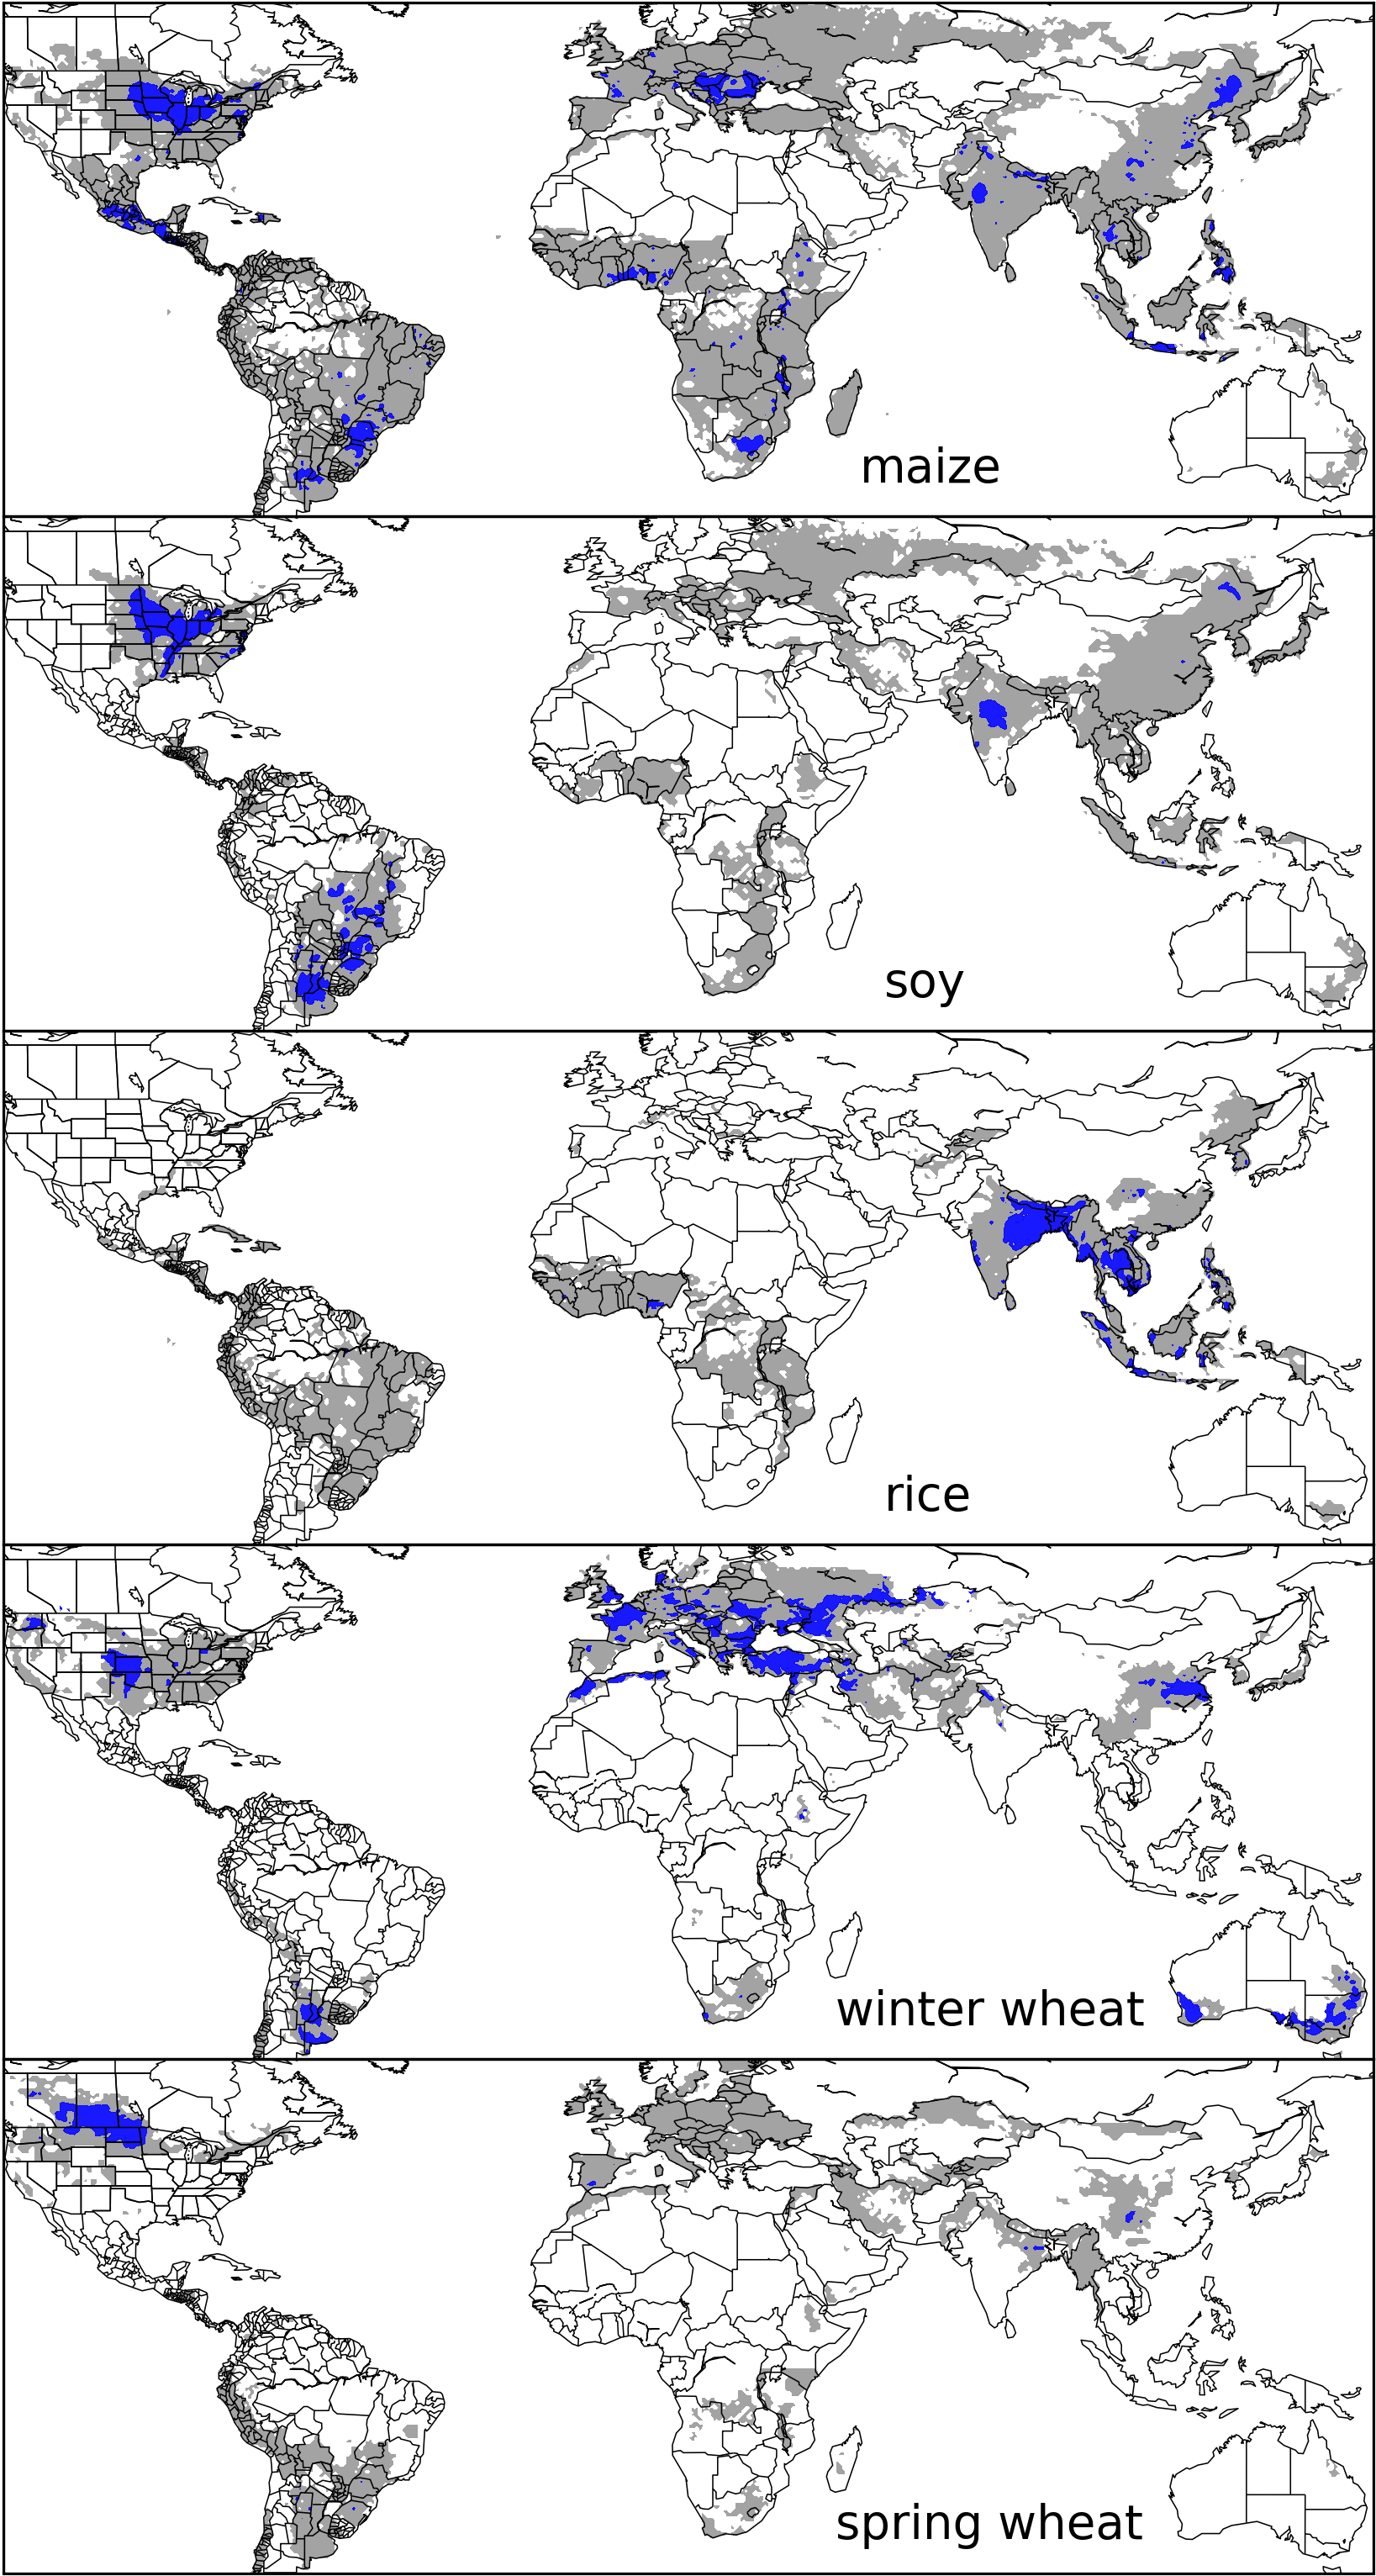
\includegraphics[width=0.95\linewidth]{figures/croparea.png}
   \caption{Presently cultivated area for rain-fed crops in the real world. Blue contour area indicates grid cells with more that 20,00 hectares (approx.\ 10\% of the land in a grid cell near the equator for example) of crop cultivated. Gray contour shows area with more that 10 hectares cultivated. Cultivated areas for maize, rice, and soy are taken from the MIRCA2000 (``monthly irrigated and rain-fed crop areas around the year 2000'') dataset \citep{Portmann2010}. Areas for winter and spring wheat areas are adapted from MIRCA2000 data and sorted by growing season. For analogous figure of irrigated crops, see Figure \ref{fig:irrarea}.}
   \label{fig:crop_area}
\end{figure}

\begin{table*}[!b]
    \small \centering
    \begin{tabular}[0.75\linewidth]{lccc} 
        \hline \vspace{1mm}
        \textbf{Input variable} & \textbf{Abbr.} & \textbf{Tested range} & \textbf{Unit}\\ \hline \hline \vspace{1mm}
        {CO$_2$}& {C} & {360, 510, 660, 810} & {ppm}\\ \hline \vspace{1mm}
        {Temperature}& {T} & {-1, 0, 1, 2, 3, 4, 5*, 6} & {$^{\circ}$C}\\ \hline \vspace{1mm}
        {Precipitation}& {W} & {-50, -30, -20, -10, 0, 10, 20, 30, (and W$_{inf}$)} & {\%}\\ \hline \vspace{1mm}
        {Applied nitrogen}& {N} & {10, 60, 200} & {kg ha$^{-1}$}\\ \hline
    \end{tabular}\\
    \parbox{11cm}{\caption{Phase II input variable test levels. Temperature and precipitation values indicate the perturbations from the historical, climatology. * Only simulated by one model. W-percentage does not apply to the irrigated (W$_{inf}$) simulations.}}
    \label{table:inputs}
\end{table*}

Statistical emulation of crop simulations has been used to combine advantageous features of both statistical and process-based models. The statistical representation of complicated numerical simulation \citep[e.g.][]{OHAGAN2006, OHAGAN2010}, in which simulation output acts as the training data for a statistical model, has been of increasing interest with the growth of simulation complexity and volume of output. Such emulators or ``surrogate models'' have been used in a variety of fields including hydrology \citep{Razavi2012}, engineering \citep{STORLIE2009}, environmental sciences \citep{RATTO2012}, and climate \citep{Castruccio14}. For agricultural impacts studies, emulation of process-based models allows exploring crop yields in regions outside ranges of current cultivation and with input variables outside historical precedents, in a lightweight, flexible form that is compatible with economic studies. 

In the past decade, many studies have developed emulators of crop yields from process-based models. Early studies proposing or describing potential emulators include \citet{Howden2005, raisen2006, Lobell2010, Iizumi2010, Ferrise2011, RUANE2013a}. Studies developing single-model emulators include \citet{Holzkamper2012} for the CropSyst model and \citet{Oyebamiji15} for the LPJmL model (for multiple crops, using multiple scenarios as a training set). In recent years, emulators have begun to be used in the context of multi-model intercomparisons, with \citet{BLANC2015, BLANC2017, Ostberg2018, Mistry2017} using them to analyze the 5 crop models of the Inter-Sectoral Impacts Model Intercomparison Project (ISIMIP) \citep{Warszawski3228} (for maize, soy, wheat, and rice). Approaches differ: \citet{BLANC2015} and \citet{BLANC2017} used local weather variables (and CO2 values) and yields but emulate across broad soil types using a single climate scenario (over multiple climate models); \citet{Ostberg2018}, used global mean temperature change (and CO$_2$) as regressors but pattern-scale to emulate local yields using multiple climate scenarios; \citet{Mistry2017} use local temperatures and yields and a historical simulation and compare with data; The first four emulate year-over-year yield variations. Other studies have used emulators to analyze non-realistic simulations that sampled a suite of climate perturbations (as opposed to RCPs): \citet{Markowski2015, Snyder2018} for temperature, water, and CO2, and \citep{FRONZEK20182} for temperature and water, both simulating selected sites for a limited number of crops.

The Global Gridded Crop Model Intercomparison (GGCMI) Phase II experiment seeks to provide a comprehensive dataset to allow systematically exploring how crop models respond to major climate and management drivers and their interactions. The experiment involves running a suite of process-based crop models across historical conditions perturbed by a set of defined input parameters, and was conducted as part of the Agricultural Model Intercomparison and Improvement Project (AgMIP) \citep{ROSENZWEIG2013, Rosenzweig2014}, an international effort conducted under a framework similar to the Climate Model Intercomparison Project (CMIP) {\citep{Taylor2012, Eyring2016}. The GGCMI protocol builds on the AgMIP Coordinated Climate-Crop Modeling Project (C3MP) \citep{ruane2014, mcdermid2015} and will contribute to the AgMIP Coordinated Global and Regional Assessments (CGRA) \citep{ruane2018, rosenzweig2018}. 

GGCMI Phase II is designed to allow addressing goals such as understanding where highest-yield regions may shift under climate change; exploring future adaptive management strategies; understanding how interacting parameters affect crop yield; quantifying uncertainties across models and major drivers; and testing strategies for producing lightweight emulators of process-based models. In this paper, we describe the GGCMI Phase II experiments, summarize output and present initial results, demonstrate that it is tractable to emulation, and present a simple climatological emulator as a potential tool for impacts assessments.

\section{Materials and Methods}
\label{S:2}
\subsection{GGCMI Phase II: experiment design}
GGCMI Phase II is the continuation of a multi-model comparison exercise begun in 2014. The initial Phase I compared harmonized yields of 21 models for 19 crops over a historical (1980-2010) scenario with a primary goal of model evaluation \citep{Elliott2015, muller_global_2017}. Phase II compares simulations of 12 models for 5 crops (maize, rice, soybean, spring wheat, and winter wheat) over hundreds of scenarios in which individual climate or management inputs are adjusted from their historical values. The reduced set of crops includes the three major global cereals and the major legume and accounts for over 50\% of human calories (in 2016, nearly 3.5 billion tons or 32\% of total global crop production by weight \citep{FAOSTAT}. 

\begin{table*}[!t]
    \small \centering
    \begin{tabular}{p{7cm} | p{1cm} p{1cm} p{1cm} p{1cm} p{1cm} p{1cm} | p{1.5cm}}
        \hline
        \textbf{Model (Key Citations)} & \textbf{Maize} & \textbf{Soy} & \textbf{Rice} & \textbf{Winter Wheat} & \textbf{Spring Wheat} & \textbf{N Dim.} & \textbf{Simulations per Crop}\\ \hline \hline
        {\textbf{APSIM-UGOE},    \citet{KEATING2003267, HOLZWORTH2014327}} & {X} & {X} & {X} & {--} & {X} & {Yes} & {37}\\ \hline
        {\textbf{CARAIB},        \citet{Dury2011, Pirttioja2015}} & {X} & {X} & {X} & {X} & {X} & {No} & {224}\\ \hline
        {\textbf{EPIC-IIASA},    \citet{BALKOVIC2014}} & {X} & {X} & {X} & {X} & {X} & {Yes} & {35}\\  \hline
        {\textbf{EPIC-TAMU},     \citet{Izaurralde06}} & {X} & {X} & {X} & {X} & {X} & {Yes} & {672}\\ \hline
        {\textbf{JULES*},        \citet{Osborne2015, Williams2015, Williams2017}} & {X} & {X} & {X} & {--} & {X} & {No} & {224}\\ \hline
        {\textbf{GEPIC},         \citet{LIU2007478, FOLBERTH201221}} & {X} & {X} & {X} & {X} & {X} & {Yes} & {384}\\ \hline
        {\textbf{LPJ-GUESS},     \citet{Lindeskog2013, Olin2015}} & {X} & {--} & {--} & {X} & {X} & {Yes} & {672}\\  \hline
        {\textbf{LPJmL},         \citet{von_Bloh_implementing_2018}} & {X} & {X} & {X} & {X} & {X} & {Yes} & {672}\\ \hline
        {\textbf{ORCHIDEE-crop}, \citet{Valade2013}} & {X} & {--} & {X} & {--} & {X} & {Yes} & {33}\\ \hline
        {\textbf{pDSSAT},        \citet{Elliott2014b, JONES2003235}} & {X} & {X} & {X} & {X} & {X} & {Yes} & {672}\\ \hline
        {\textbf{PEPIC},         \citet{LIU2016164, LIU2016}} & {X} & {X} & {X} & {X} & {X} & {Yes} & {130}\\ \hline
        {\textbf{PROMET*\dag},       \citet{MAUSER2009362, Hank2015, MAUSER2015}} & {X} & {X} & {X} & {X} & {X} & {Yes\dag} & {239}\\ \hline \hline
        {Totals} & {12} & {10} & {11} & {9} & {12} & {--} & {3993 (maize)}\\
        \hline
    \end{tabular}
 \caption{Models included in the GGCMI Phase II and the number of C, T, W, and N simulations performed for rain-fed crops (``Sims per Crop''), with 672 as the maximum. ``N-Dim.'' indicates if simulations include varying nitrogen levels; two models omit this dimension. All models provided the same set of simulations across all modeled crops, but some omitted individual crops in some cases. (For example, APSIM did not simulate winter wheat.) Irrigated simulations are provided at the level of the other covariates for each model (for an additional 84 simulations for the fully-sampled models). Geographic extent of simulation varies to some extent within a certain model for different scenarios (672 rain-fed simulations does not necessarily equal 672 climatological yields in all areas). This geographic variance only applies for areas far outside the area of currently cultivated crops. Two models (marked with *) use non-AgMERRA climate inputs. For further details on models, see \citet{Elliott2015}. \dag PROMET provided simulations at only two nitrogen levels so is not emulated across the nitrogen dimension.} 
\label{table:models}
\end{table*}

The major goals of GGCMI Phase II are to:
\begin{itemize}
  \setlength\itemsep{0.3mm}
    \item Enhance understanding of how models work by characterizing their sensitivity to input climate and nitrogen drivers.
    \item Study the interactions between climate variables and nitrogen inputs in driving modeled yield impacts. 
    \item Explore differences in crop response to warming across the Earth's climate regions.
    \item Provide a dataset that allows statistical emulation of crop model responses for downstream modelers.
    \item Illustrate differences in potential adaptation via growing season changes. 
\end{itemize}

The guiding scientific rationale of GGCMI Phase II is to provide a comprehensive, systematic evaluation of the response of process-based crop models to different values for carbon dioxide, temperature, water, and applied nitrogen (collectively known as ``CTWN''). Phase II of the GGCMI project consists of a series of simulations, each with one or more of the CTWN dimensions perturbed over the 31-year historical time series (1980-2010) used in Phase I. In most cases, historical daily climate inputs are taken from the 0.5 degree NASA AgMERRA daily gridded re-analysis product specifically designed for agricultural modeling, with satellite-corrected precipitation \citep{Ruane2015}. Two models require sub-daily input data and use alternative sources. See \citet{Elliott2015} for additional details. 

The experimental protocol consists of 9 levels for precipitation perturbations, 7 for temperature, 4 for CO$_2$, and 3 for applied nitrogen, for a total of 672 simulations for rain-fed agriculture and an additional 84 for irrigated (Table \ref{table:inputs}). For irrigated simulations, soil water is held at either field capacity or, for those models that include water-log damage, at maximum beneficial level.  Temperature perturbations are applied as absolute offsets from the daily mean, minimum, and maximum temperature time series for each grid cell used as inputs. Precipitation perturbations are applied as fractional changes at the grid cell level, and carbon dioxide and nitrogen levels are specified as discrete values applied uniformly over all grid cells. Note that CO$_2$ changes are applied independently of changes in climate variables, so that higher CO$_2$ is not associated with higher temperatures. An additional, identical set of scenarios (at the same C, T, W, and N levels) simulate adaptive agronomy under climate change by varying the growing season for crop production. (These adaptation simulations are not shown or analyzed here.) The resulting GGCMI data set captures a distribution of crop responses over the potential space of future climate conditions.

The 12 models included in GGCMI Phase II are all mechanistic process-based crop models that are widely used in impacts assessments (Table \ref{table:models}). Although some of the models shares a common base (e.g. LPJmL and LPJ-GUESS and the EPIC models), they have developed independently from this shared base, for more details on the genealogy of the models see Figure S1 in \citet{Rosenzweig2014}. Differences in model structure does mean that several key factors are not standardized across the experiment, including secondary soil nutrients, carry over effects across growing years including residue management and soil moisture, and extent of simulated area for different crops. Growing seasons are identical across models, but vary by crop and by location on the globe. All stresses except factors related to nitrogen, temperature, and water (e.g. Alkalinity, salinity) are disabled. No additional nitrogen inputs, such as atmospheric deposition, are considered, but some models have individual assumptions on soil organic matter that may release additional nitrogen through mineralization. See \citet{Rosenzweig2014}, \citet{Elliott2015} and \citet{muller_global_2017} for further details on models and underlying assumptions.

Each model is run at 0.5 degree spatial resolution and covers all currently cultivated areas and much of the uncultivated land area.  Coverage extends considerably outside currently cultivated areas because cultivation will likely shift under climate change. See Figure \ref{fig:crop_area} for the present-day cultivated area of rain-fed crops, and Figure \ref{fig:irrarea} in the supplemental material for irrigated crops. Some areas such as Greenland, far-northern Canada, Siberia, Antarctica, the Gobi and Sahara deserts, and central Australia are not simulated as they are assumed to remain non-arable even under an extreme climate change. Growing seasons are standardized across models with data adapted from several sources \citep{Sacks2010, Portmann2008, Portmann2010}.

The participating modeling groups provide simulations at any of four initially specified levels of participation, so the number of simulations varies by model, with some sampling only a part of the experiment variable space. Most modeling groups simulate all five crops in the protocol, but some omitted one or more. Table \ref{table:models} provides details of coverage for each model. Note that the three models that provide less than 50 simulations are excluded from the emulator analysis. 

All models produce as output, crop yields (tons ha$^{-1}$ year$^{-1}$) for each 0.5 degree grid cell. Because both yields and yield changes vary substantially across models and across grid cells, we primarily analyze relative change from a baseline. We take as the baseline the scenario with historical climatology (i.e.\ T and P changes of 0). C of 360 ppm, and applied N at 200 kg ha$^-1$.  We show absolute yields in some cases to illustrate geographic differences in yields for a single model. 

\subsection{Simulation model validation approach}
%%%%%%%%%%%%%%
%%Needs Work%%
%%%%%%%%%%%%%%
Simulation model validation for GGCMI phase II builds on the validation efforts presented in \citet{muller_global_2017} for the first phase. In the case presented here however, the models are not run on the best approximation of management levels (namely nitrogen application level) by country as with phase I. As the goals of this phase of the project are focused on understanding the sensitivity in \textit{change} in yield to changes in input drivers --and not to simulate historical yields as accurately as possible-- no direct comparison to historical yield data can be made. Additionally, even when provided with an appropriate local nitrogen level, models simulated \textit{potential} yields that do not included reductions from pests, weeds, or diseases. Potential yields represent an ideal case that is not realized in many less industrialized areas. Finally, some models are not calibrated as they were in phase I of the project.

We evaluate the models here based on the response to year-to-year temperature and precipitation variability in the historical record. If the models can (somewhat) faithfully represent the the historical variability in yields (which, once detrended to account for changing management levels must be driven largely by differences in weather), then the models may provide some utility in understanding the impact on mean climatological shifts in temperature and precipitation. Specifically, we calculate a Pearson correlation coefficient between the detrended time series of simulations and FAO data for the period 1981-2009. Validating the response to CO$_2$ and Nitrogen applications is more difficult because real world data is not available outside of small greenhouse and field level trials.

\subsection{Climatological-mean yield emulator design}
\begin{figure}[!h]
\centering
   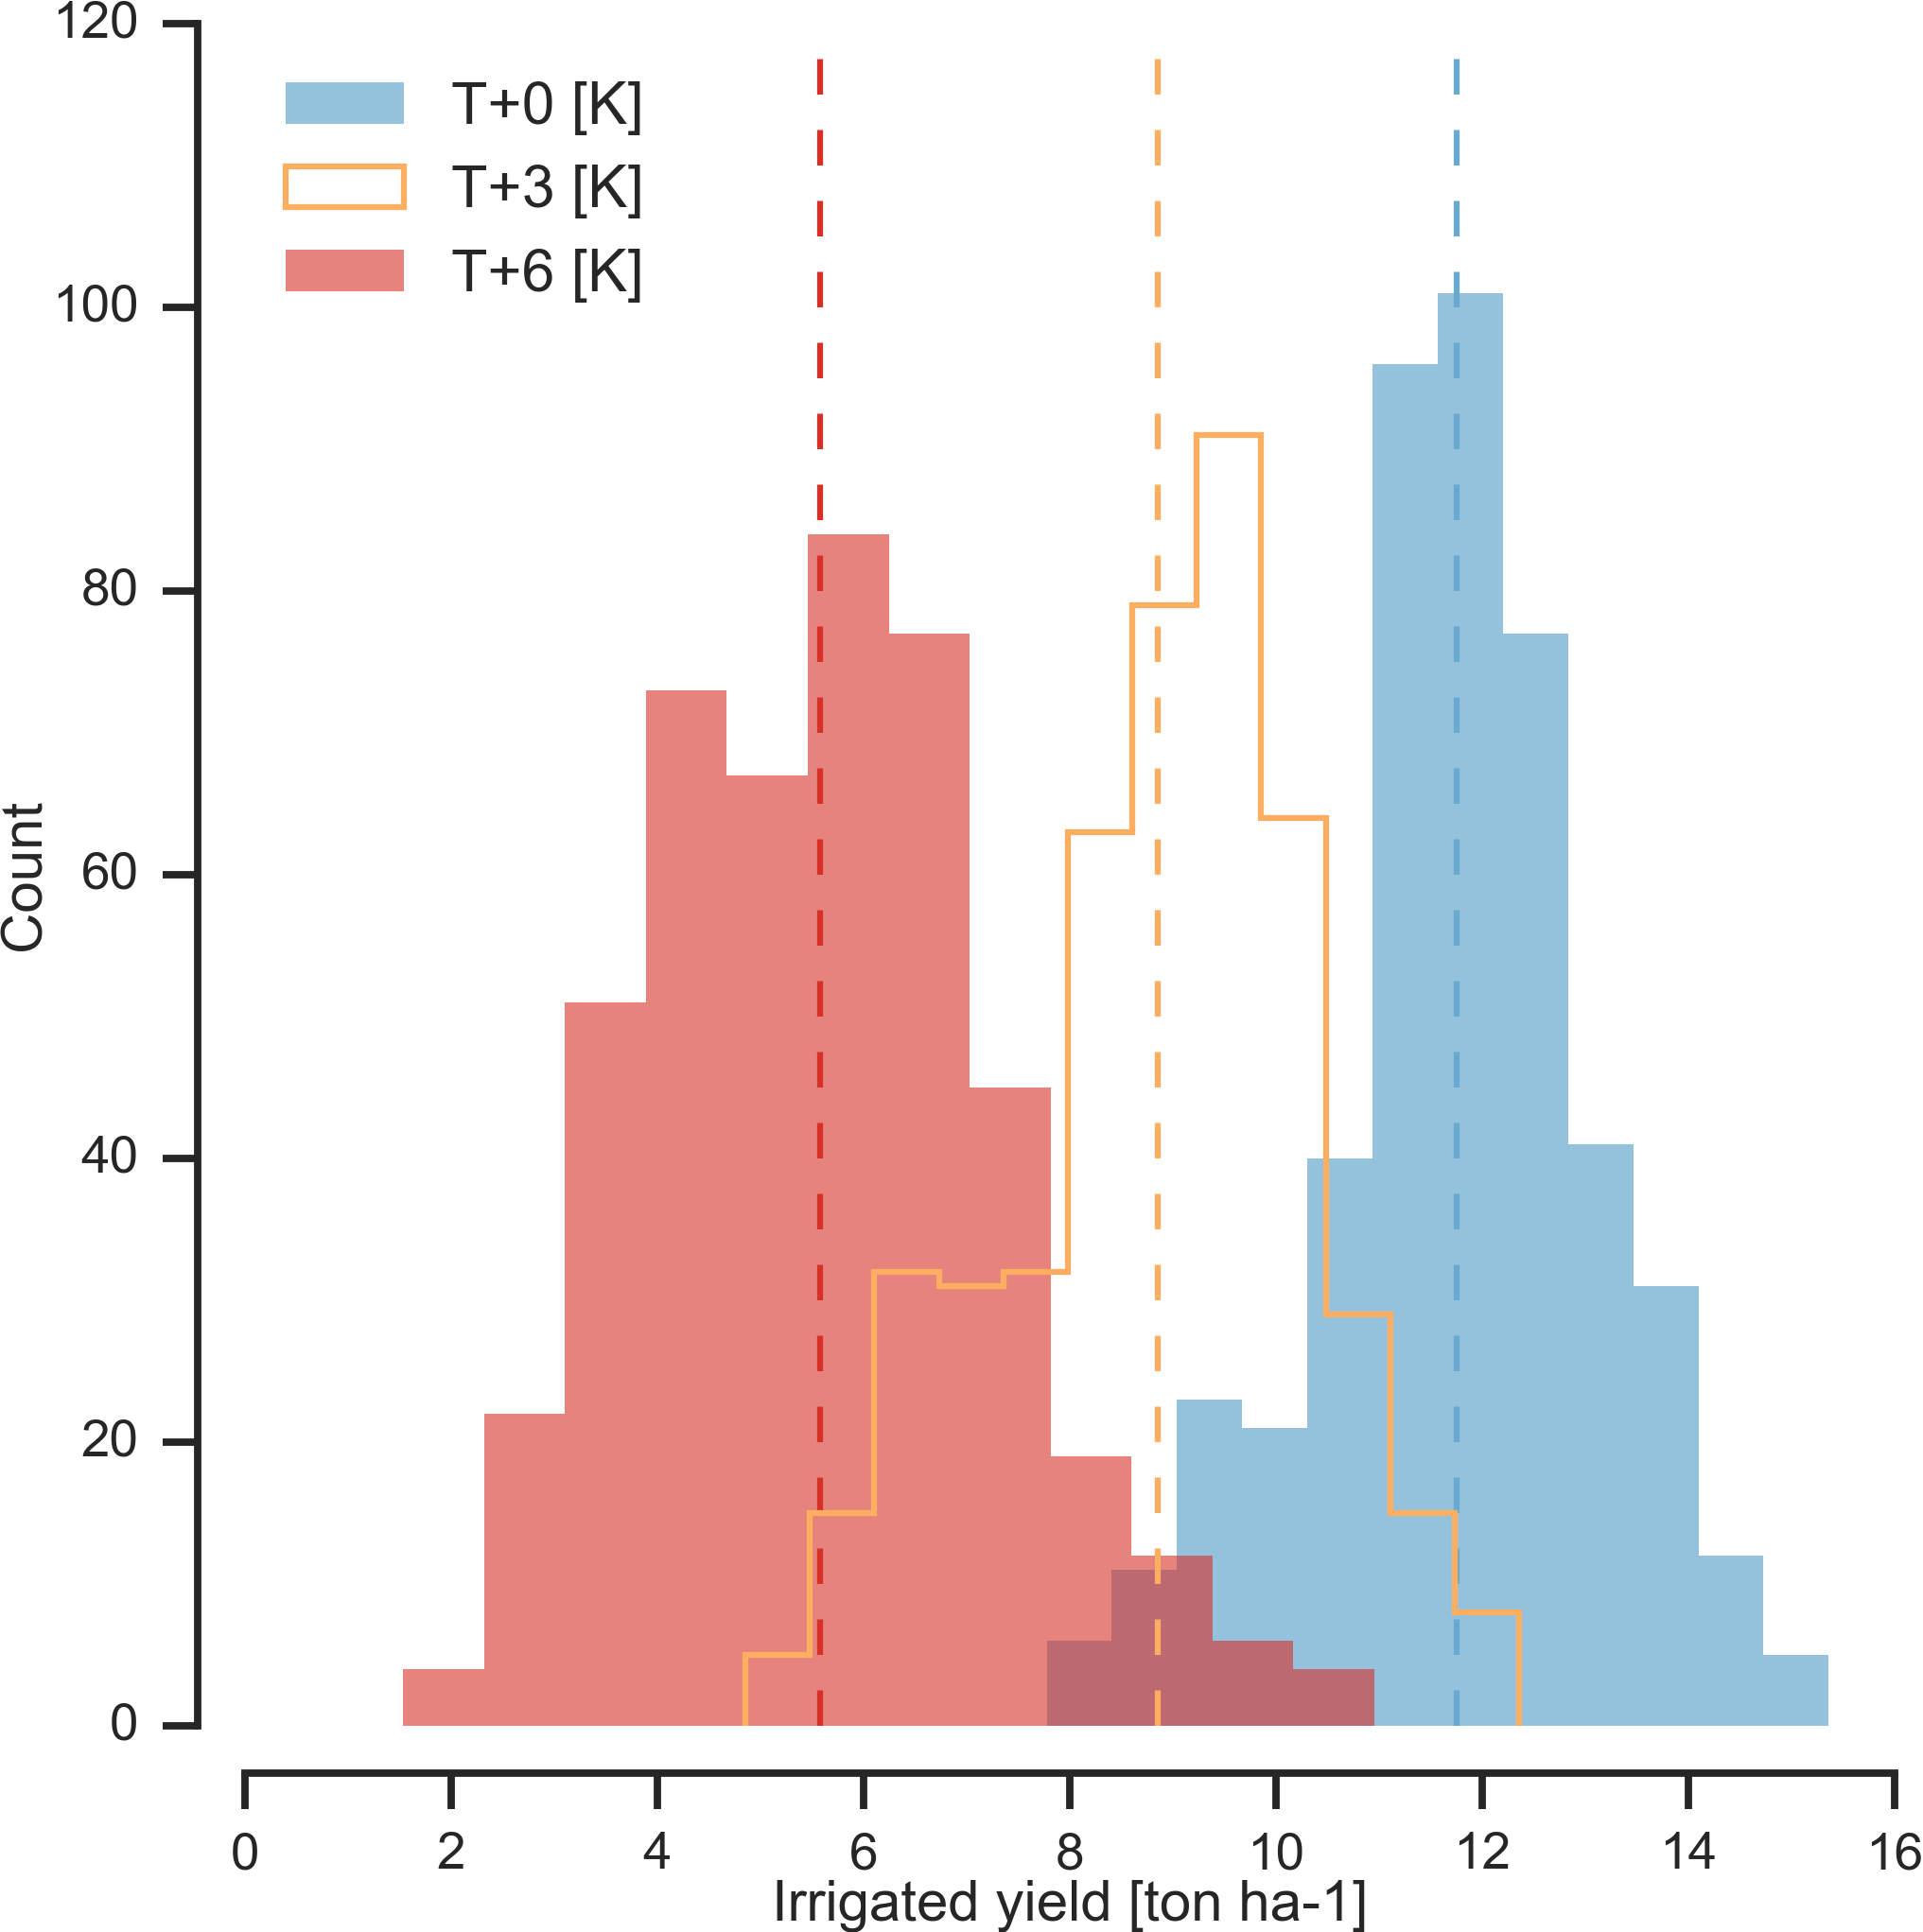
\includegraphics[width=0.95\linewidth]{figures/hist_year.png}
   \caption{Example showing both climatological mean yields and distribution of yearly yields for three 30-year scenarios. Figure shows rain-fed maize for a grid cell in northern Iowa (a representative high-yield region) from the pDSSAT model, for the baseline climatology (1981-2010) and for scenarios with temperature shifted by (T) +3 and (T) +6 $^{\circ}$C, with other variables held at baseline values. Dashed vertical lines and black dots indicate the climatological mean yield.}
   \label{fig:yearly}
\end{figure}

\begin{figure*}[!b]
\centering
   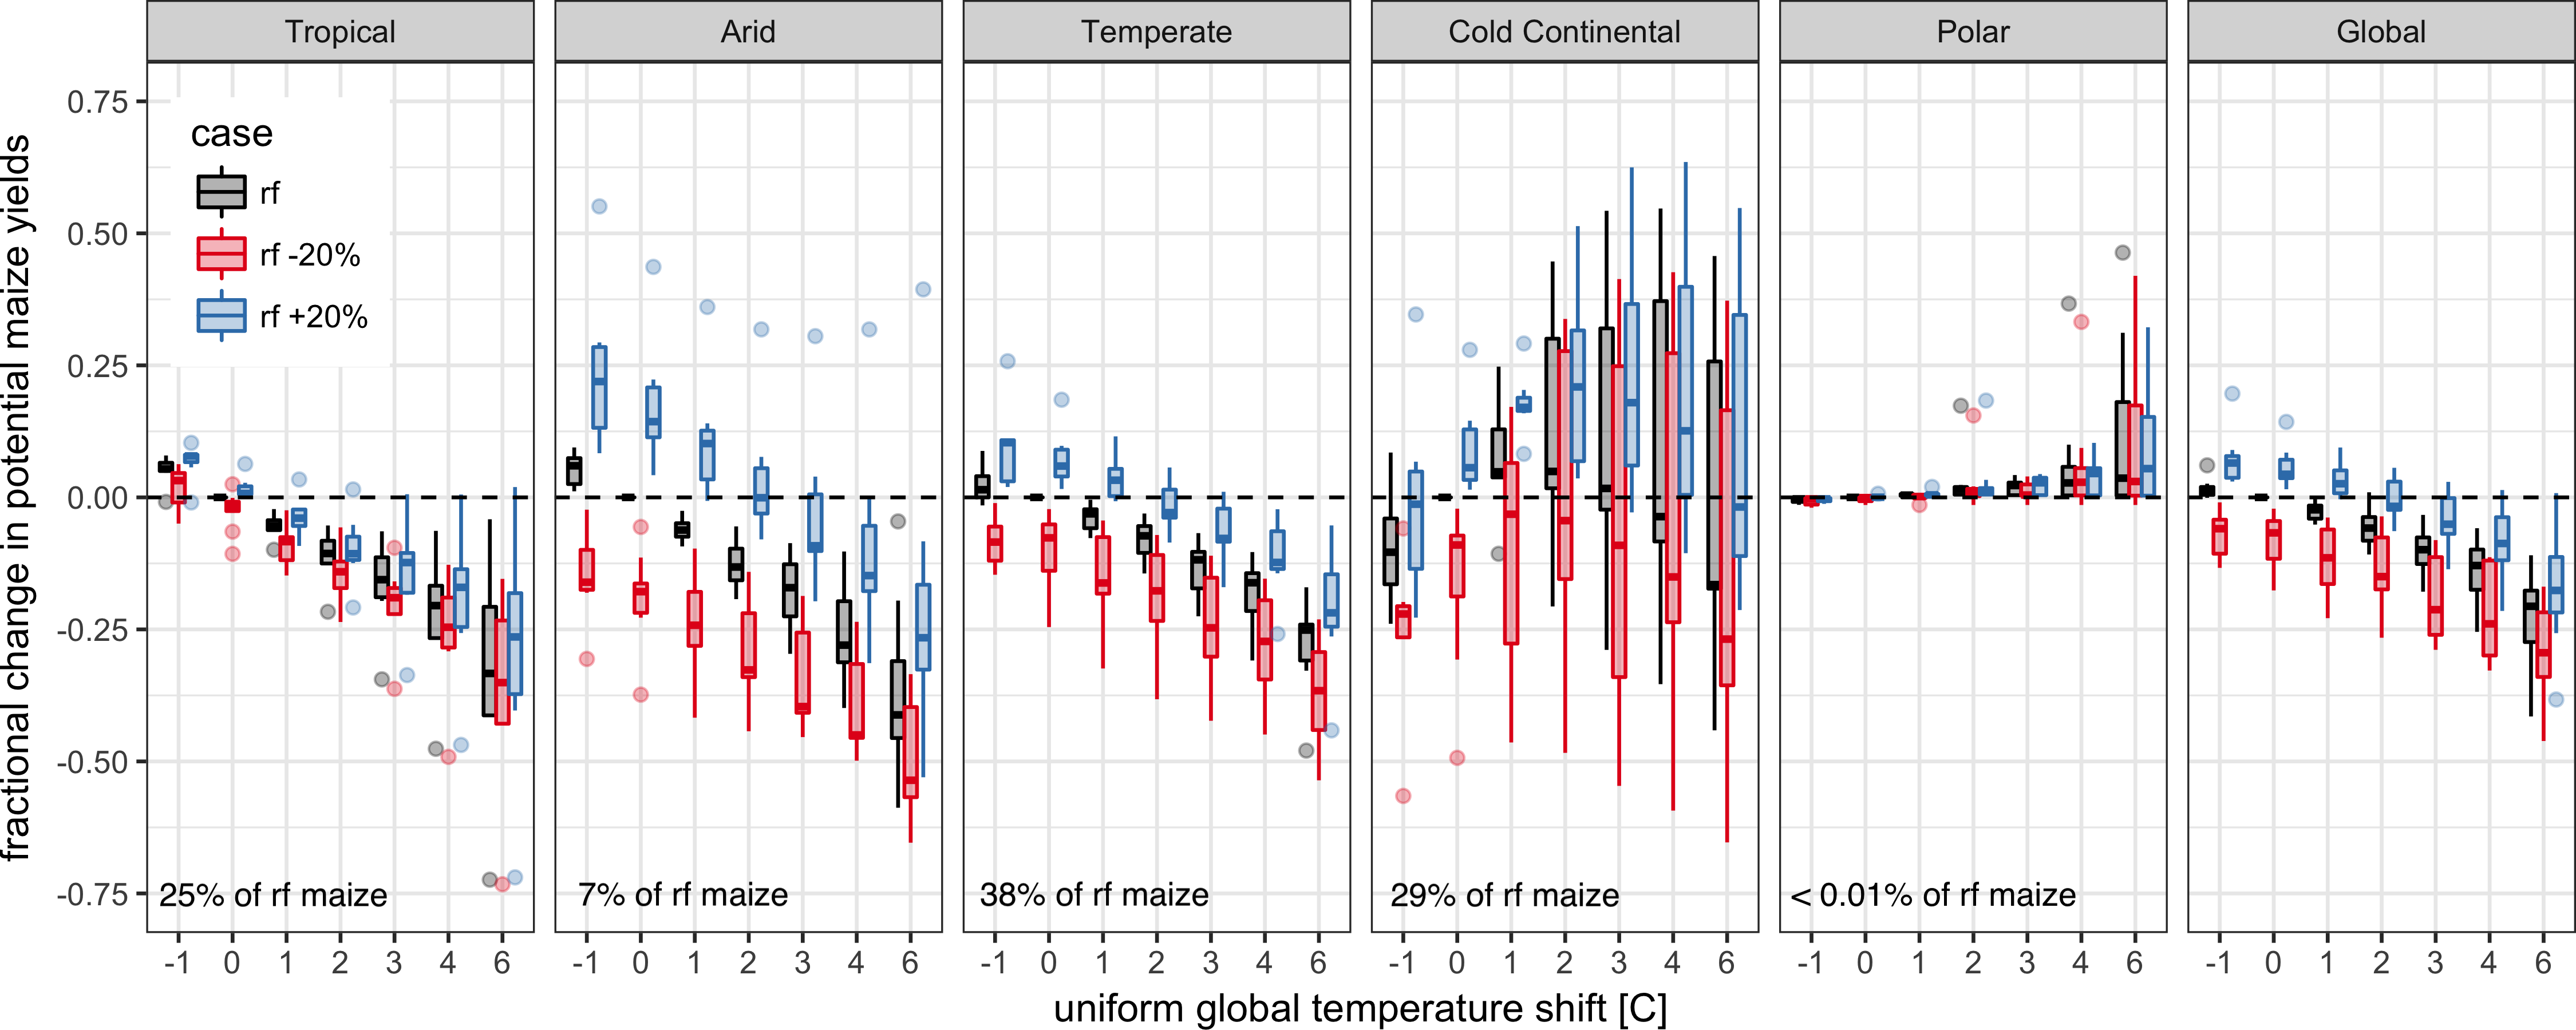
\includegraphics[width=0.95\linewidth]{figures/global_sim_CG.png}
   \caption{Illustration of the distribution of regional yield changes across the multi-model ensemble, split by K\"{o}ppen-Geiger climate regions (\cite{rubel2010}).
    We show responses of a single crop (rain-fed maize) to applied uniform temperature perturbations, for three discrete precipitation perturbation levels (rain-fed (rf) -20\%, rain-fed (0), and rain-fed +20\%), with CO$_2$ and nitrogen held constant at baseline values (360 pmm and 200 kg ha$^{-1}$ yr$^{-1}$). Y-axis is fractional change in the regional average climatological potential yield relative to the baseline. The figure shows all modeled land area; see Figure \ref{fig:KGirr_currentcult} in the supplemental material for only currently-cultivated land. Panel text gives the percentage of rain-fed maize presently cultivated in each climate zone \citep{Portmann2010}. Box-and-whiskers plots show distribution across models, with median marked. Box edges are first and third quartiles, i.e.\ box height is the interquartile range (IQR). Whiskers extend to maximum and minimum of simulations but are limited at 1.5$\cdot$IQR; otherwise the outlier is shown. Models generally agree in most climate regions (other than cold continental), with projected changes larger than inter-model variance. Outliers in the tropics (strong negative impact of temperature increases) are the pDSSAT model; outliers in the high-rainfall case (strong positive impact of precipitation increases) are the JULES model. Inter-model variance increases in the case where precipitation is reduced, suggesting uncertainty in model response to water limitation. The right panel with global changes shows yield responses to an globally uniform temperature shift; note that these results are not directly comparable to simulations of more realistic climate scenarios with the same global mean change.}
   \label{fig:globesim}
\end{figure*}

We construct our emulator at the 30-year climatological mean level. \citet{BLANC2015} and \citet{BLANC2017} have shown that a emulator of a global process-based crop simulation model can be successfully developed at the yearly scale. 

The decision to first construct a climatological-mean yield emulator is driven by the target application for this analysis tool. Many impact modelers are not focused on the changes in the year-to-year variability in yields, but instead on the broad mean changes over the multi-decadal timescale. Emulation involves fitting individual regression models for each crop, simulation model, and 0.5 degree geographic pixel from the GGCMI Phase II data set. The regressors are the applied constant perturbations in temperature, water, nitrogen and CO$_2$, we aggregate the simulation outputs in the time dimension, and regress on the 30-year mean yields. (See Figure \ref{fig:yearly} for illustration). The regression therefore omits information about yield responses to year-to-year climate perturbations, which are more complex. Emulating inter-annual yield variations would likely require considering statistical details of the historical climate time series, including changes in marginal distribution and temporal dependencies. (Future work should explore this). The climatological emulation indirectly includes any yield response to geographically distributed factors such as soil type, insolation, and the baseline climate itself, because we construct separate emulators for each grid cell. The emulator parameter matrices are portable and the yield computations are cheap even at the half-degree grid cell resolution, so we do not aggregate in space at this time.

\citet{BLANC2015} and \citet{BLANC2017} have shown that a fractional polynomial specification is more effective than a standard polynomial for representing simulations at the yearly level across different soil types geographically (not at the grid cell level). We do not test this specification here, and instead use as a starting point a standard third-order polynomial to represent the climatological-mean response at the grid cell level as it is the simplest effective specification. 

We regress climatological-mean yields against a third-order polynomial in C, T, W, and N with interaction terms. The higher-order terms are necessary to capture any nonlinear responses, which are well-documented in observations for temperature and water perturbations (e.g.\ \citet{Schlenker2009} for T and \citet{He2016} for W). We include interaction terms (both linear and higher-order) because past studies have shown them to be significant effects. For example, \citet{Lobell2007} and \citet{Tebaldi2008} showed that in real-world yields, the joint distribution in T and W is needed to explain observed yield variance (C and N are fixed in these data). Other observation-based studies have shown the importance of the interaction between water and nitrogen \citep[e.g.][]{AULAKH2005}, and between nitrogen and carbon dioxide \citep{Mitsuru92, Nakamura97}. We do not focus on comparing different model specifications in this study, and instead stick to a relatively simple parameterized specification that allows for some, albeit limited, coefficient interpretation. 

The limited GGCMI variable sample space means that use of the full polynomial expression described above, which has 34 terms for the rain-fed case (12 for irrigated), can be problematic, and can lead to over-fitting and unstable parameter estimations. We therefore reduce the number of terms through a feature selection cross-validation process in which terms in the polynomial are tested for importance. In this procedure higher-order and interaction terms are added successively to the model; we then follow the reduction of the the aggregate mean squared error with increasing terms and eliminate those terms that do not contribute significant reductions. See supplemental documents for more details. We select terms by applying the feature selection process to the three models that provided the complete set of 672 rain-fed simulations (pDSSAT, EPIC-TAMU, and LPJmL); the resulting choice of terms is then applied for all emulators. 

Feature importance is remarkably consistent across all three models and across all crops (see Figure \ref{fig:featureselection} in the supplemental material). The feature selection process results in a final polynomial in 23 terms, with 11 terms eliminated. We omit the N$^3$ term, which cannot be fitted because we sample only three nitrogen levels. We eliminate many of the C terms: the cubic, the CT, CTN, and CWN interaction terms, and all higher order interaction terms in C.  Finally, we eliminate two 2nd-order interaction terms in T and one in W. Implication of this choice include that nitrogen interactions are complex and important, and that water interaction effects are more nonlinear than those in temperature. The resulting statistical model (Equation \ref{eqn:features_final}) is used for all grid cells, models, and crops: 

\begin{align}
    \label{eqn:features_final}
    Y\ = \ & K_{1}  \\
       + \ & K_{2}  C     + K_{3}  T     + K_{4}  W     + K_{5}  N   \nonumber \\
       + \ & K_{6}  C^2   + K_{7}  T^2   + K_{8}  W^2   + K_{9}  N^2 \nonumber \\
       + \ & K_{10} C W   + K_{11} C N   + K_{12} T W   + K_{13} T N + K_{14} W N \nonumber \\ % lost 1 term, CT
       + \ & K_{15} T^3   + K_{16} W^3   + K_{17} T W N  \nonumber \\ % lost 2 terms, C^3 and N^3
       + \ & K_{18} T^2 W + K_{19} W^2 T + K_{20} W^2 N  \nonumber \\ % lost 2 terms, CWN and CTN
       + \ & K_{21} N^2 C + K_{22} N^2 T + K_{23} N^2 W  \nonumber    % lose 6 terms: T^2N and T^2C, W^2C, 3 C^2 terms
\end{align}

To fit the parameters $K$, we use a Bayesian Ridge probabilistic estimator \citep{MacKay91}, which reduces volatility in parameter estimates when the sampling is sparse, by weighting parameter estimates towards zero. The Bayesian Ridge method is necessary to maintain a consistent functional form across all models, and locations as the linear least squares fails to provide a stable result in many cases. In the GGCMI Phase II experiment, the most problematic fits are those for models that provided a limited number of cases or for low-yield geographic regions where some modeling groups did not run all scenarios. Because we do not attempt to emulate models that provided less than 50 simulations, the lowest number of simulations emulated across the full parameter space is 130 (for the PEPIC model). We use the implementation of the Bayesian Ridge estimator from the scikit-learn package in Python \citep{scikit-learn}. 

The resulting parameter matrices for all crop model emulators are available on request, as are the raw simulation data and a Python application to emulate yields. The yield output for a single GGCMI model that simulates all scenarios and all five crops is $\sim$12.5 GB; the emulator is $\sim$100 MB, a reduction by over two orders of magnitude. 

\begin{figure*}[!htb]
\centering
   \includegraphics[width=0.95\linewidth]{figures/baselinecomp_yield_3.png} 
   \caption{Illustration of the spatial pattern of potential yields and potential yield changes in the GGCMI Phase II ensemble, for three major crops. Left column (a) shows multi-model mean climatological yields for the baseline scenario for (top--bottom) rain-fed maize, soy, and rice. (For wheat see Figure \ref{fig:wheatbaseline} in the supplemental material.) White stippling indicates areas where these crops are not currently cultivated. Absence of cultivation aligns well with the lowest yield contour (0-2 ton ha$^{-1}$). Right column (b) shows the multi-model mean fractional yield change in the extreme T + 4 $^{\circ}$C scenario (with other inputs at baseline values). Areas without hatching or stippling are those where confidence in projections is high: the multi-model mean fractional change exceeds two standard deviations of the ensemble. ($\Delta > 2\sigma$). Hatching indicates areas of low confidence ($\Delta < 1 \sigma$), and stippling areas of medium confidence ($1 \sigma < \Delta < 2 \sigma$). Crop model results in cold areas, where yield impacts are on average positive, also have the highest uncertainty.}
   \label{fig:maizesoybaseline}
\end{figure*}

\subsection{Emulator evaluation}
Because no general criteria exist for defining an acceptable model emulator, we develop a metric of emulator performance specific to GGCMI. For a multi-model comparison exercise like GGCMI, a reasonable criterion is what we term the ``normalized error'', which compares the fidelity of an emulator for a given model and scenario to the inter-model uncertainty. We define the normalized error $e$ for each scenario as the difference between the fractional yield change from the emulator and that in the original simulation, divided by the standard deviation of the multi-model spread (Equations \ref{eqn:per_yield} and  \ref{eqn:error}):

\begin{equation}
    \label{eqn:per_yield}
    F_{\: scn.}=\frac{Y_{scn.}-Y_{baseline}}{Y_{baseline}}
\end{equation}

\begin{equation}
    \label{eqn:error}
    e_{\: scn.} =\frac{F_{em, \: scn.}-F_{sim, \: scn.}}{\sigma_{sim, \: scn.}}
\end{equation}

Here $F_{\: scn.}$ is the fractional change in a model's mean emulated or simulated yield from a defined baseline, in some scenario (scn.) in C, T, W, and N space; $Y_{scn.}$ and $Y_{baseline}$ are the absolute emulated or simulated mean yields. The normalized error $e$ is the difference between the emulated fractional change in yield and that actually simulated, normalized by $\sigma_{sim}$, the standard deviation in simulated fractional yields $F_{sim,\: scn.}$ across all models. The emulator is fit across all available simulation outputs, and then the error is calculated across the simulation scenarios provided by all nine models (Figure \ref{fig:error_360} and Figures \ref{fig:error360total} and Figures \ref{fig:error810} in supplemental documents). Note that the normalized error $e$ for a model depends not only on the fidelity of its emulator in reproducing a given simulation but on the particular suite of models considered in the intercomparison exercise. The rationale for this choice is to relate the fidelity of the emulation to an estimate of true uncertainty, which we take as the multi-model spread. 

\section{Results}
\label{S:3}
\subsection{Simulation results}
Crop models in the GGCMI ensemble show a broadly consistent responses to climate and management perturbations in most regions, with a strong negative impact of increased temperature in all but the coldest regions. We illustrate this result for rain-fed maize in Figure \ref{fig:globesim}, which shows yields for the primary K\"{o}ppen-Geiger climate regions \citep{rubel2010}. In warming scenarios, models show decreases in maize yield in the temperate, tropical, and arid regions that account for nearly three-quarters of global maize production. These impacts are robust for even moderate climate perturbations. In the temperate zone, even a 1 degree temperature rise with other variables held fixed leads to a median yield reduction that outweighs the variance across models. A 6 degree temperature rise results in median loss of $\sim$25\% of yields with a signal to noise of nearly three. A notable exception is the cold continental region, where models disagree strongly, extending even to the sign of impacts. Model simulations of other crops produce similar responses to warming, with robust yield losses in warmer locations and high inter-model variance in the cold continental regions (Figures \ref{fig:KGcrops_all}).

The effects of rainfall changes on maize yields are also as expected and are consistent across models. Increased rainfall mitigates the negative effect of higher temperatures, most strongly in arid regions. Decreased rainfall amplifies yield losses and also increases inter-model variance more strongly, suggesting that models have difficulty representing crop response to water stress.  We show only rain-fed maize here; see Figure \ref{fig:KGirr_all} for the irrigated case. As expected, irrigated crops are more resilient to temperature increases in all regions, especially so where water is limiting.  

Mapping the distribution of baseline yields and yield changes shows the geographic dependencies that underlie these results. Figure \ref{fig:maizesoybaseline} shows baseline and changes in the T+4 scenario for rain-fed maize, soy, and rice in the multi-model ensemble mean, with locations of model agreement marked.Absolute yield potentials are have strong spatial variation, with much of the Earth's surface area unsuitable for any given crop. In general, models agree most on yield response in regions where yield potentials are currently high and therefore where crops are currently grown. Models show robust decreases in yields at low latitudes, and highly uncertain median increases at most high latitudes. For wheat crops see Figure \ref{fig:wheatbaseline}; wheat projections are both more uncertain and show fewer areas of increased yield in the inter-model mean. 

\subsection{Simulation model validation results}
%%%%%%%%%%%%%%
%%Needs Work%%
%%%%%%%%%%%%%%
\begin{figure*}[!htb]
    \centering
    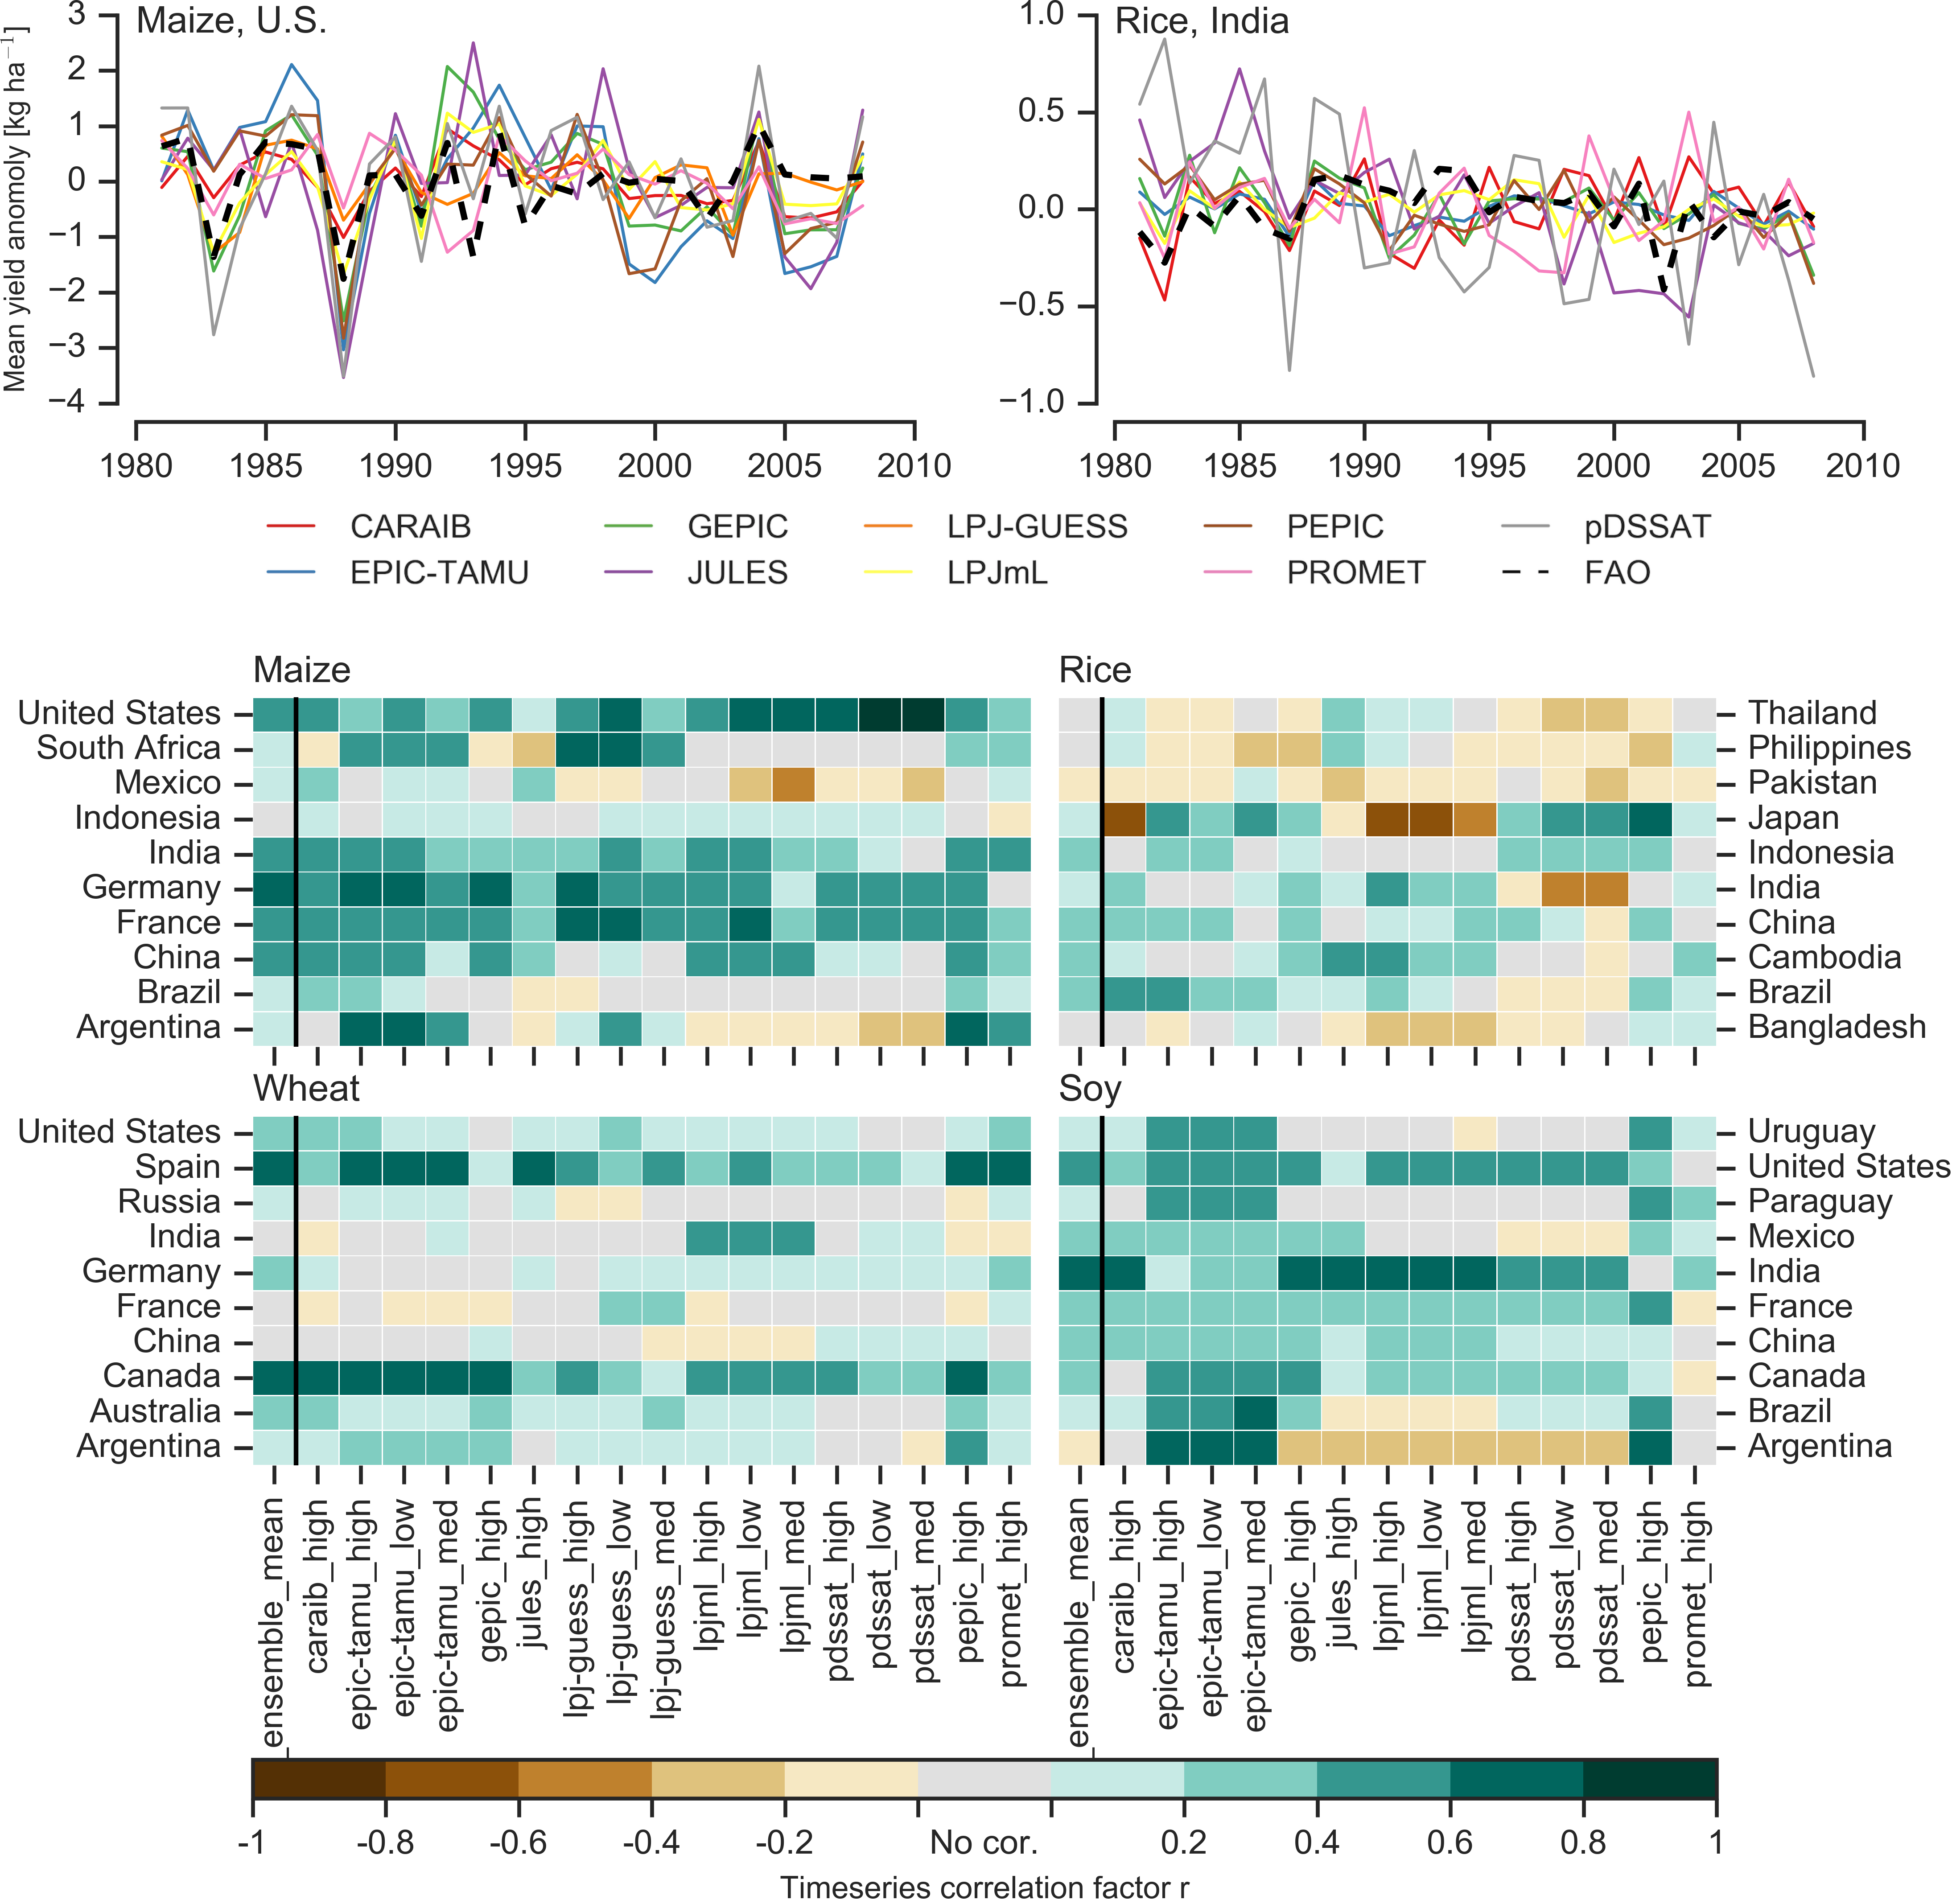
\includegraphics[width=0.95\linewidth]{figures/Agformet_validation.png}
    \caption{Time series correlation coefficients between simulated crop yield and FAO data at the country level. The top panels indicate two example cases: US maize (a good case), and rice in India (mixed case), both for the high nitrogen application case. The heatmaps illustrate the Pearson r correlation between the detrended simulation mean yield at the country level compared to the detrended FAO yield data for the top producing countries for each crop with continuous FAO data over the 1980-2010 period. Models that provided different nitrogen application levels are shown with low, med, and high label (models that did not simulated different nitrogen levels are analogous to a high nitrogen application level). The ensemble mean yield is also correlated with the FAO data.}
    \label{fig:simulation_val}
\end{figure*}

Figure \ref{fig:simulation_val} shows the time series correlation between the simulation model yield and FOA yield data. The results are mixed, with many regions for rice and wheat being difficult to model. No single model is dominant, with each model providing near best-in-class performance in at least one location-crop combination. The presence of no vertical dark green color bars clearly illustrates the power of a multi-model intercomparison project like the one presented here. The ensemble mean yield is calculated across all `high' nitrogen application level model simulations and correlated with the FAO data (not the mean of the correlations). The ensemble mean does not beat the best model in each case, but shows positive correlation in over 75\% of the cases presented here.

Soy is qualitatively the easiest crop to represent (except in Argentina), which is likely due to the invariance of the response to nitrogen application (soy fixes atmospheric nitrogen very efficiently). Comparison to the FAO data is therefore easier than the other crops because the nitrogen application levels do not matter. US maize has the best performance across models, with nearly every model representing the historical variability to some extent. Especially good example years for US maize are 1983, 1988, and 2004 (top left panel), where every model gets the direction of the anomaly compared to surrounding years correct. 1983 and 1988 are famously bad years for US maize along with 2012 (not shown). US maize is possibly both the most uniformly industrialized (in terms of management practices) crop and the one with the best data collection in the historical period of all the cases presented here.

FAO data is at least one level of abstraction from ground truth in many cases, especially in developing countries. The failure of models to represent the year-to-year variability in rice in some countries in southeast Asia is likely partly due to model failure and partly due to lack of data. Partitioning of these contributions is impossible at this stage. Additionally, there is less year-to-year variability in rice yields (partially due to the fraction of irrigated cultivation). Since the Pearson r metric is scale invariant, it will tend to score the rice models more poorly than maize and soy. The pDSSAT model shows very poor performance for rice in India (top right panel).

\textit{One may speculate that the difference in performance between Pakistan (no successful models) and India (many successful models) for rice may lie in the FAO data and not the models themselves. What would be so different about rice production across these two countries that could explain this difference??}

%\begin{figure}[!htb]
    %\centering
    %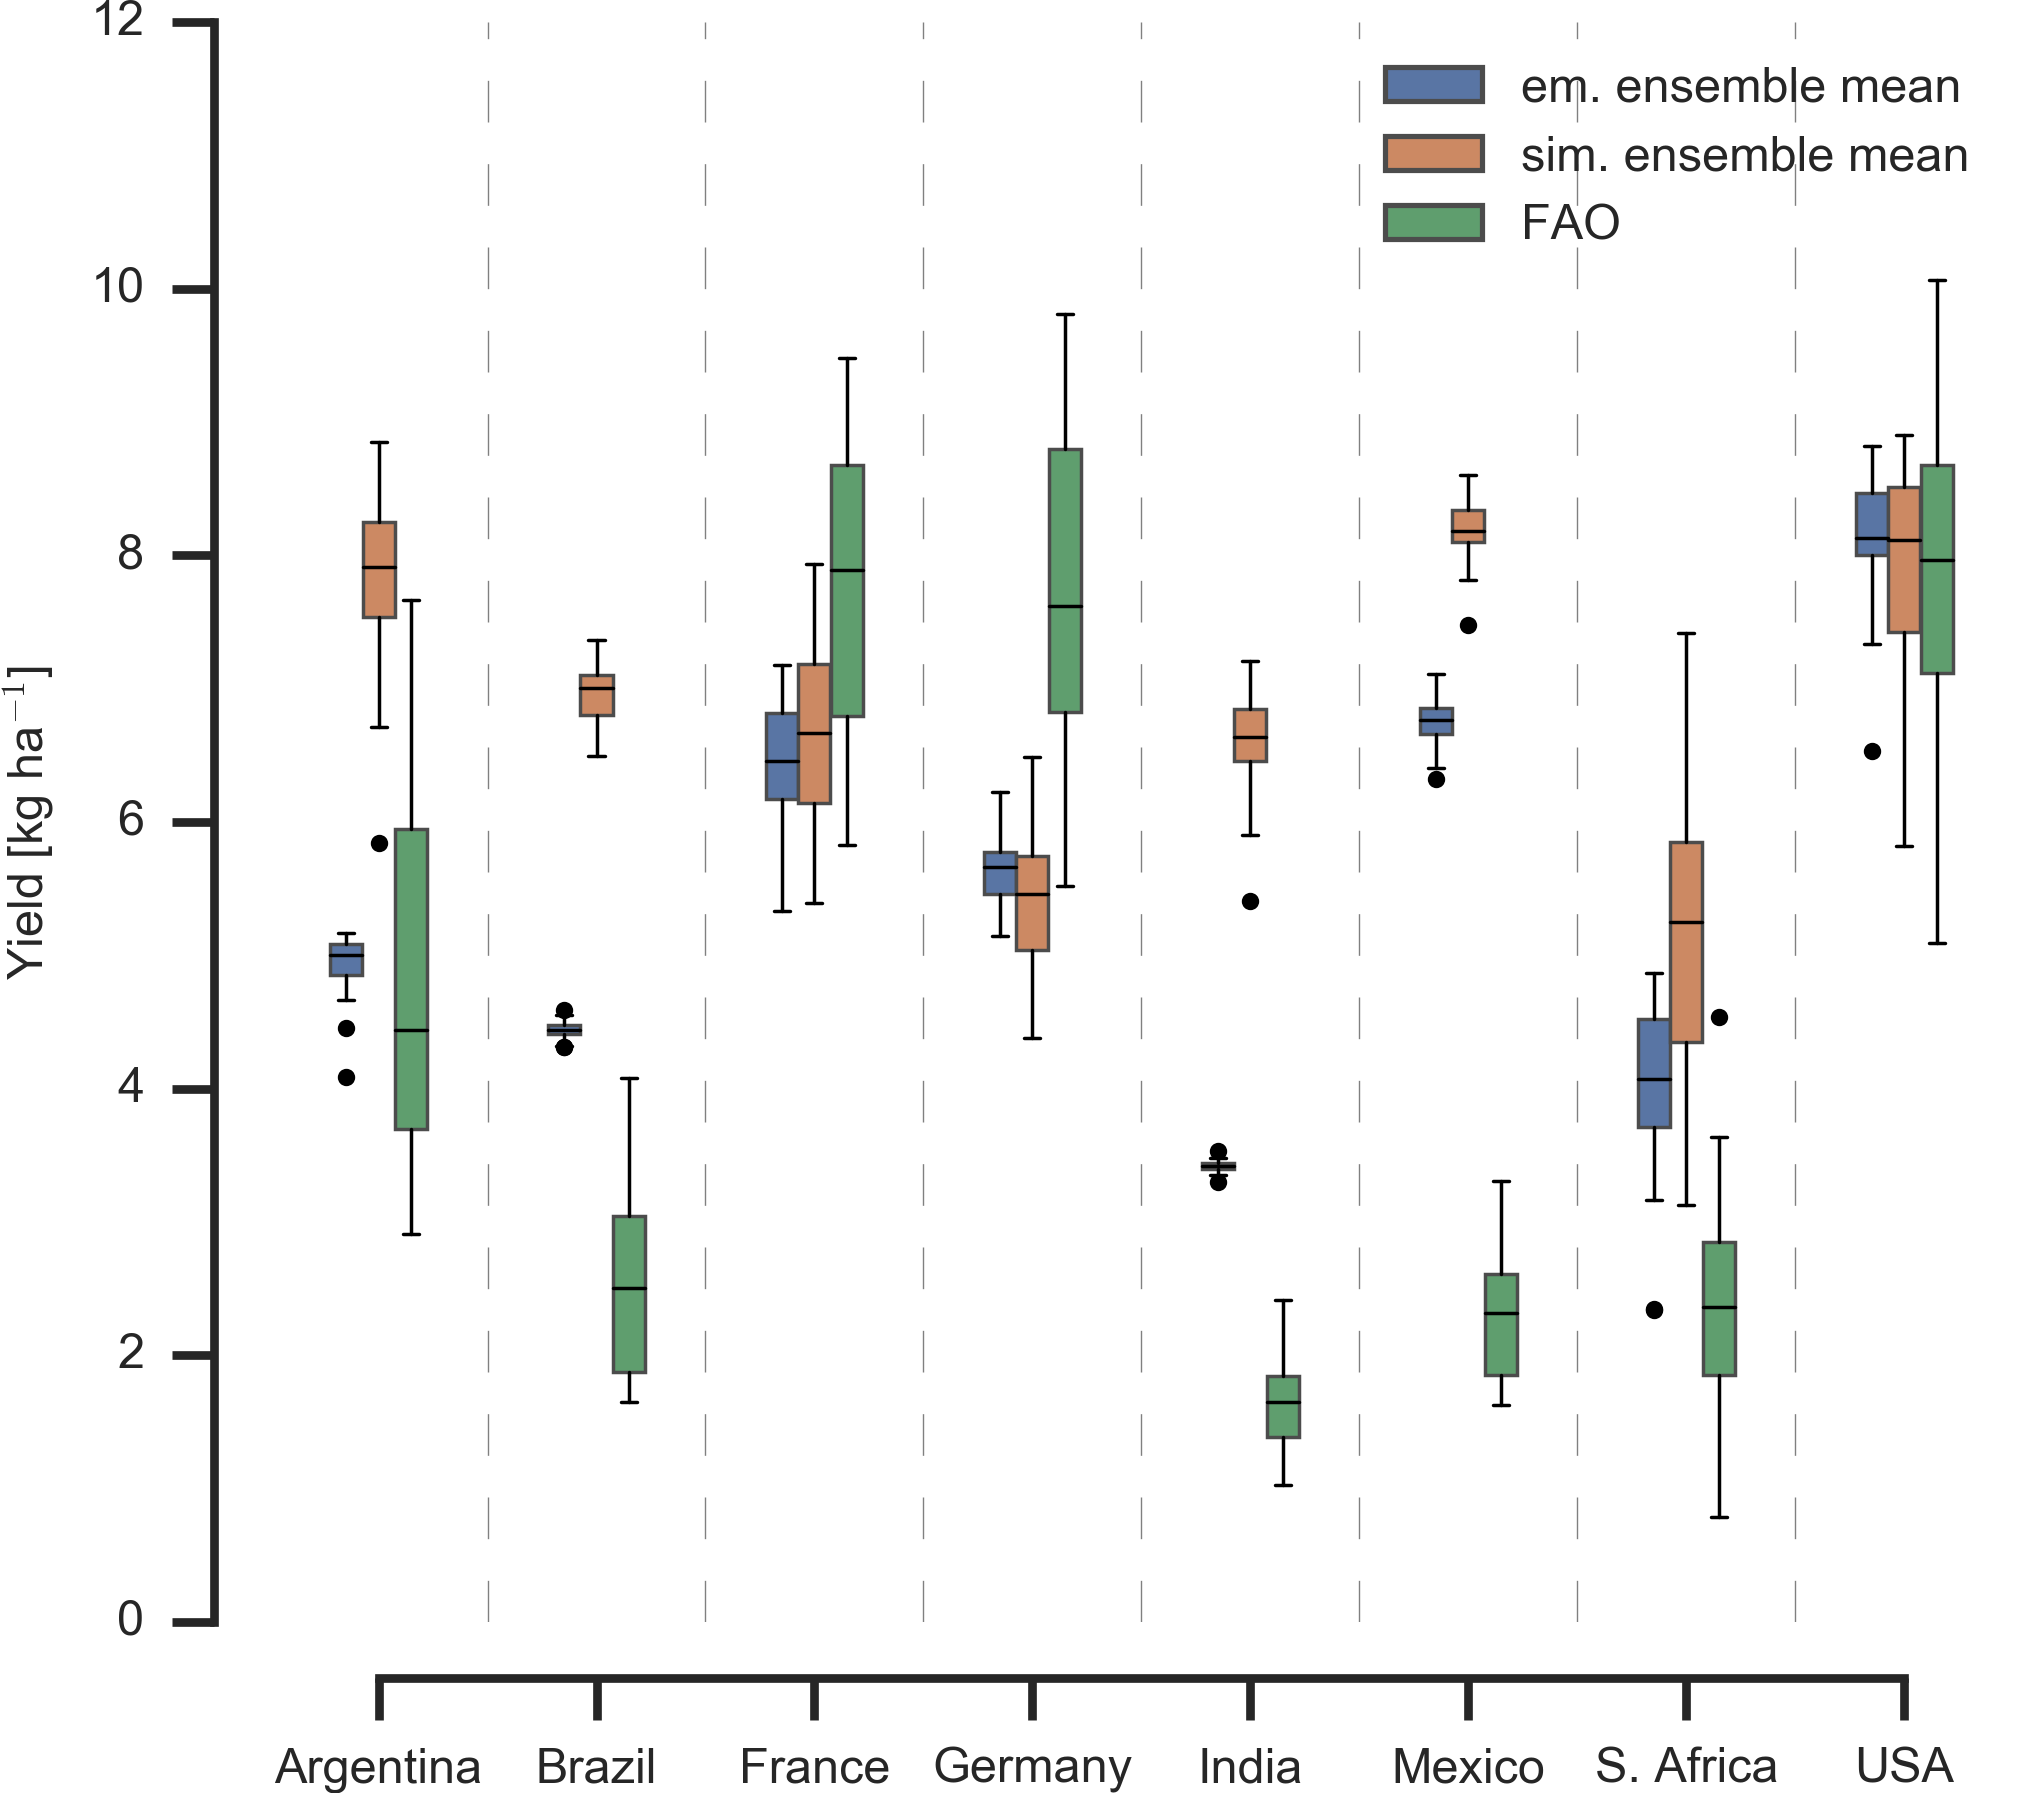
\includegraphics[width=0.98\linewidth]{figures/Agformet_validation2.png}
    %\caption{Distribution in historical yields (1981-2009) for maize for eight example high producing countries. FAO, simulation (high nitrogen), and emulation. Emulated values are calculated based on the additive temperature anomaly or percentage precipitation anomaly from the 1981-2009 period in each year. Note: the emulator is designed to provide the mean change in yield under climatological mean shift in temperature (or precipitation). Applying it at the year to year level should be interpreted with caution.}
    %\label{fig:sim_em_val}
%\end{figure}

Figure \ref{fig:sim_em_val} shows the distribution across historical maize yields for some high producing countries. The discrepancy between the simulations and FAO data is most evident in developing nations, where nitrogen application levels are far below the 200 kg ha$^-1$ applied in the simulations shown here (though the distributions are similar in those nations otherwise). The distribution in historical yields is also calculated with the climatological-mean emulator by passing it the historical (1981-2009) anomalies in growing season precipitation and temperature, CO2 concentration of 360 ppm, and spatially varying nitrogen application rates \citep[data from:~][]{potter2010, Mueller2012}. The emulator distribution is shifted towards the FAO distribution in cases where the nitrogen levels are too high in the simulations, but this does not account for 


\begin{figure*}[!h]
\centering
    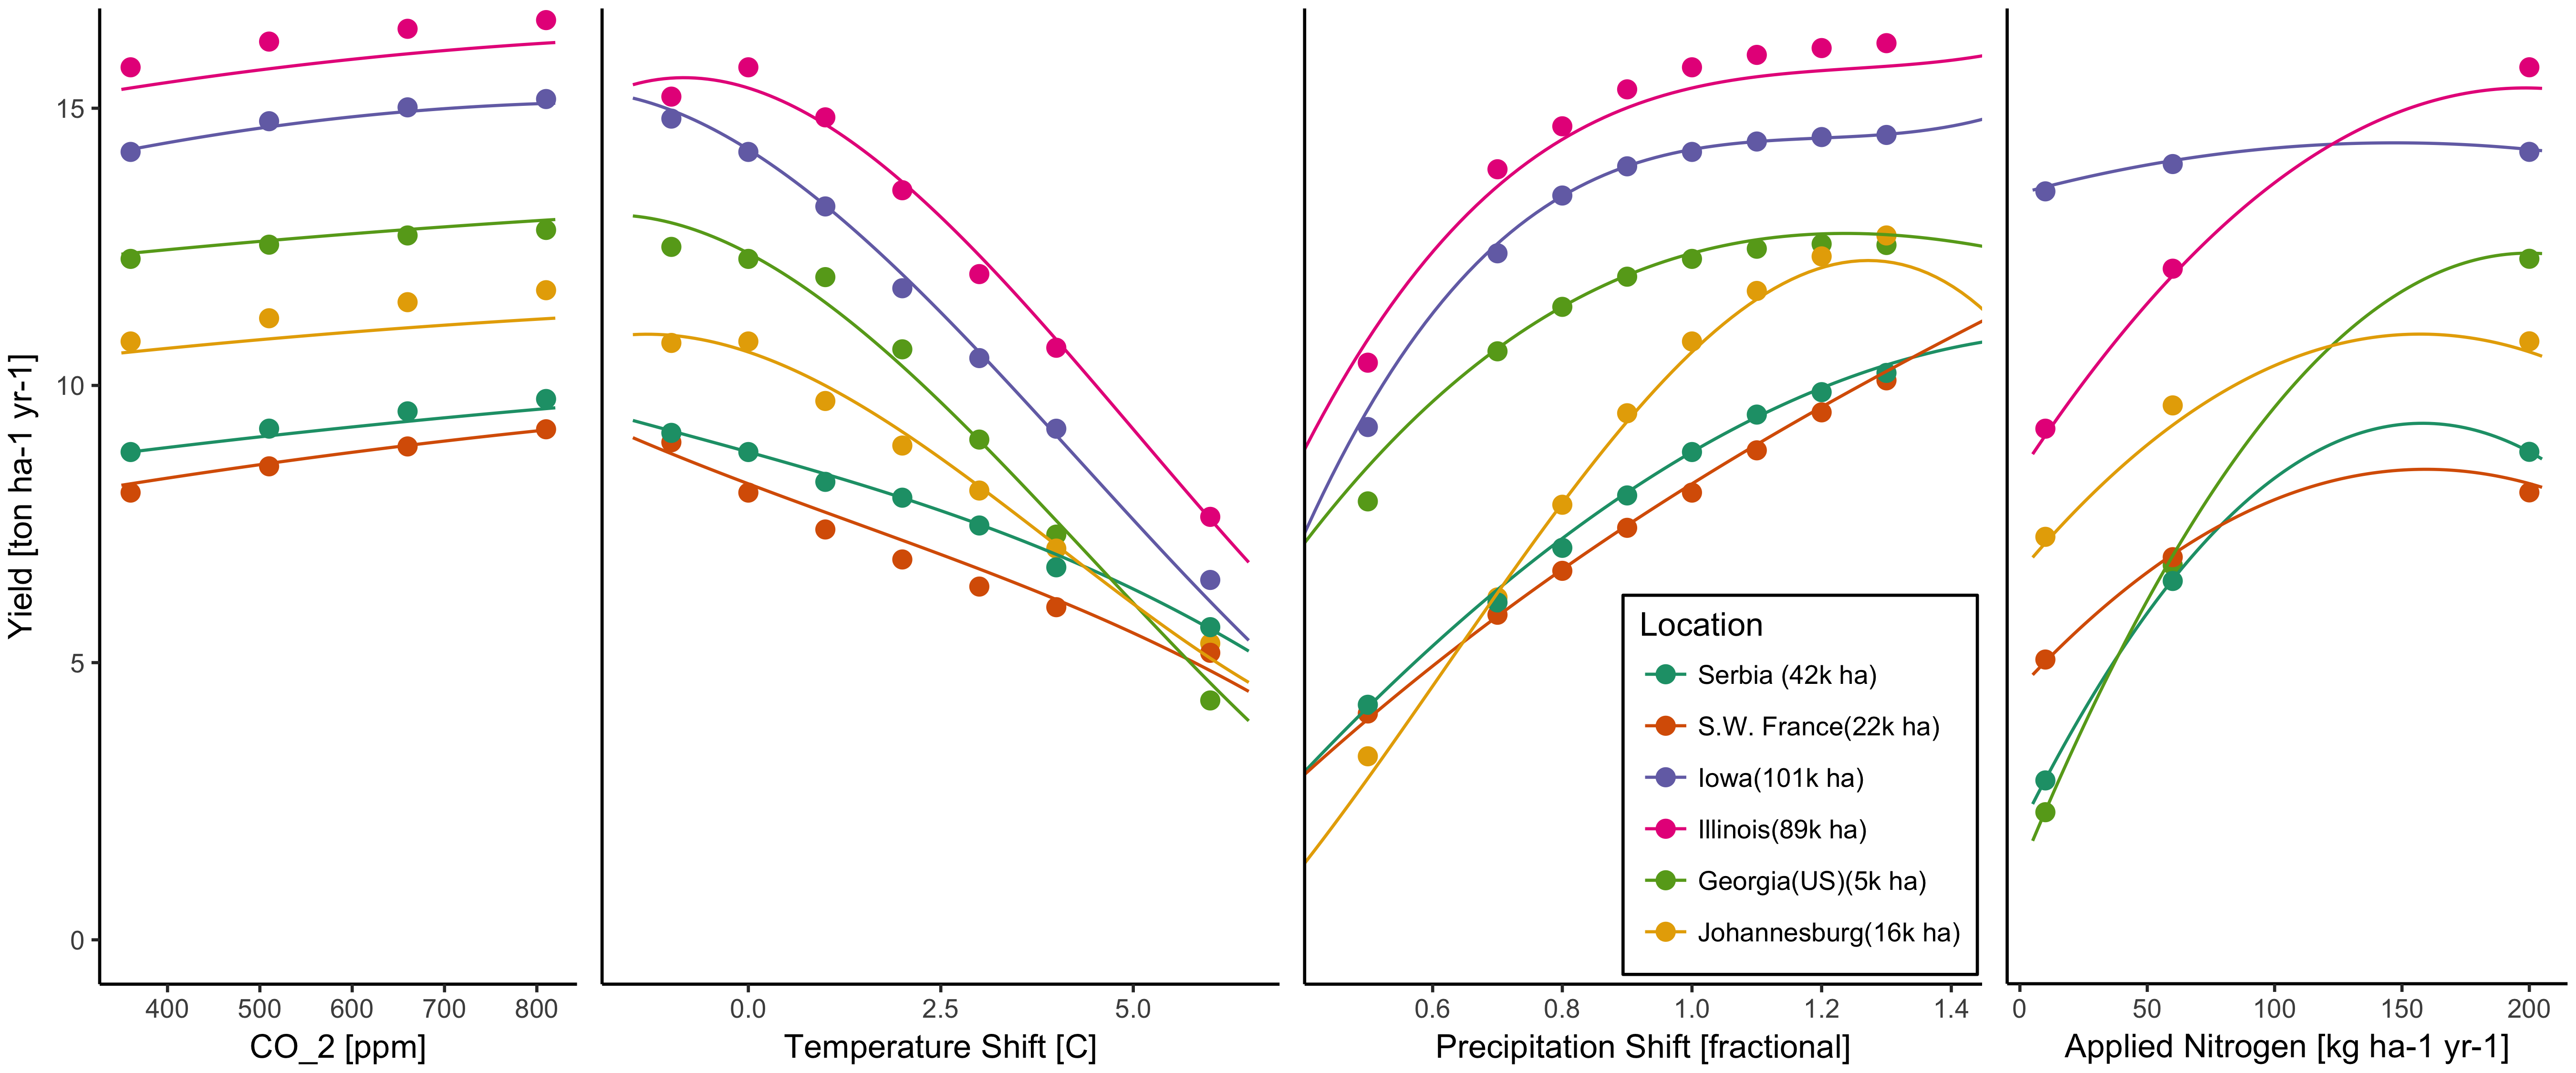
\includegraphics[width=0.95\linewidth]{figures/regression_areas.png}
    \caption{Example illustrating spatial variations in yield response and emulation ability. We show rain-fed maize in the pDSSAT model in six example locations selected to represent high-cultivation areas around the globe. Legend includes hectares cultivated in each selected grid cell. Each panel shows variation along a single variable, with others held at baseline values. Dots show climatological mean yield, solid lines a simple polynomial fit across this 1D variation, and dashed lines the results of the full emulator of Equation \ref{eqn:features_final}. The climatological response is sufficiently smooth to be be represented by a simple polynomial. Because precipitation changes are imposed as multiplicative factors rather than additive offsets, locations with higher baseline precipitation have a larger absolute spread in inputs sampled than do drier locations (not visible here).}
   \label{fig:regression}
\end{figure*}

\begin{figure*}[!h]
\centering
    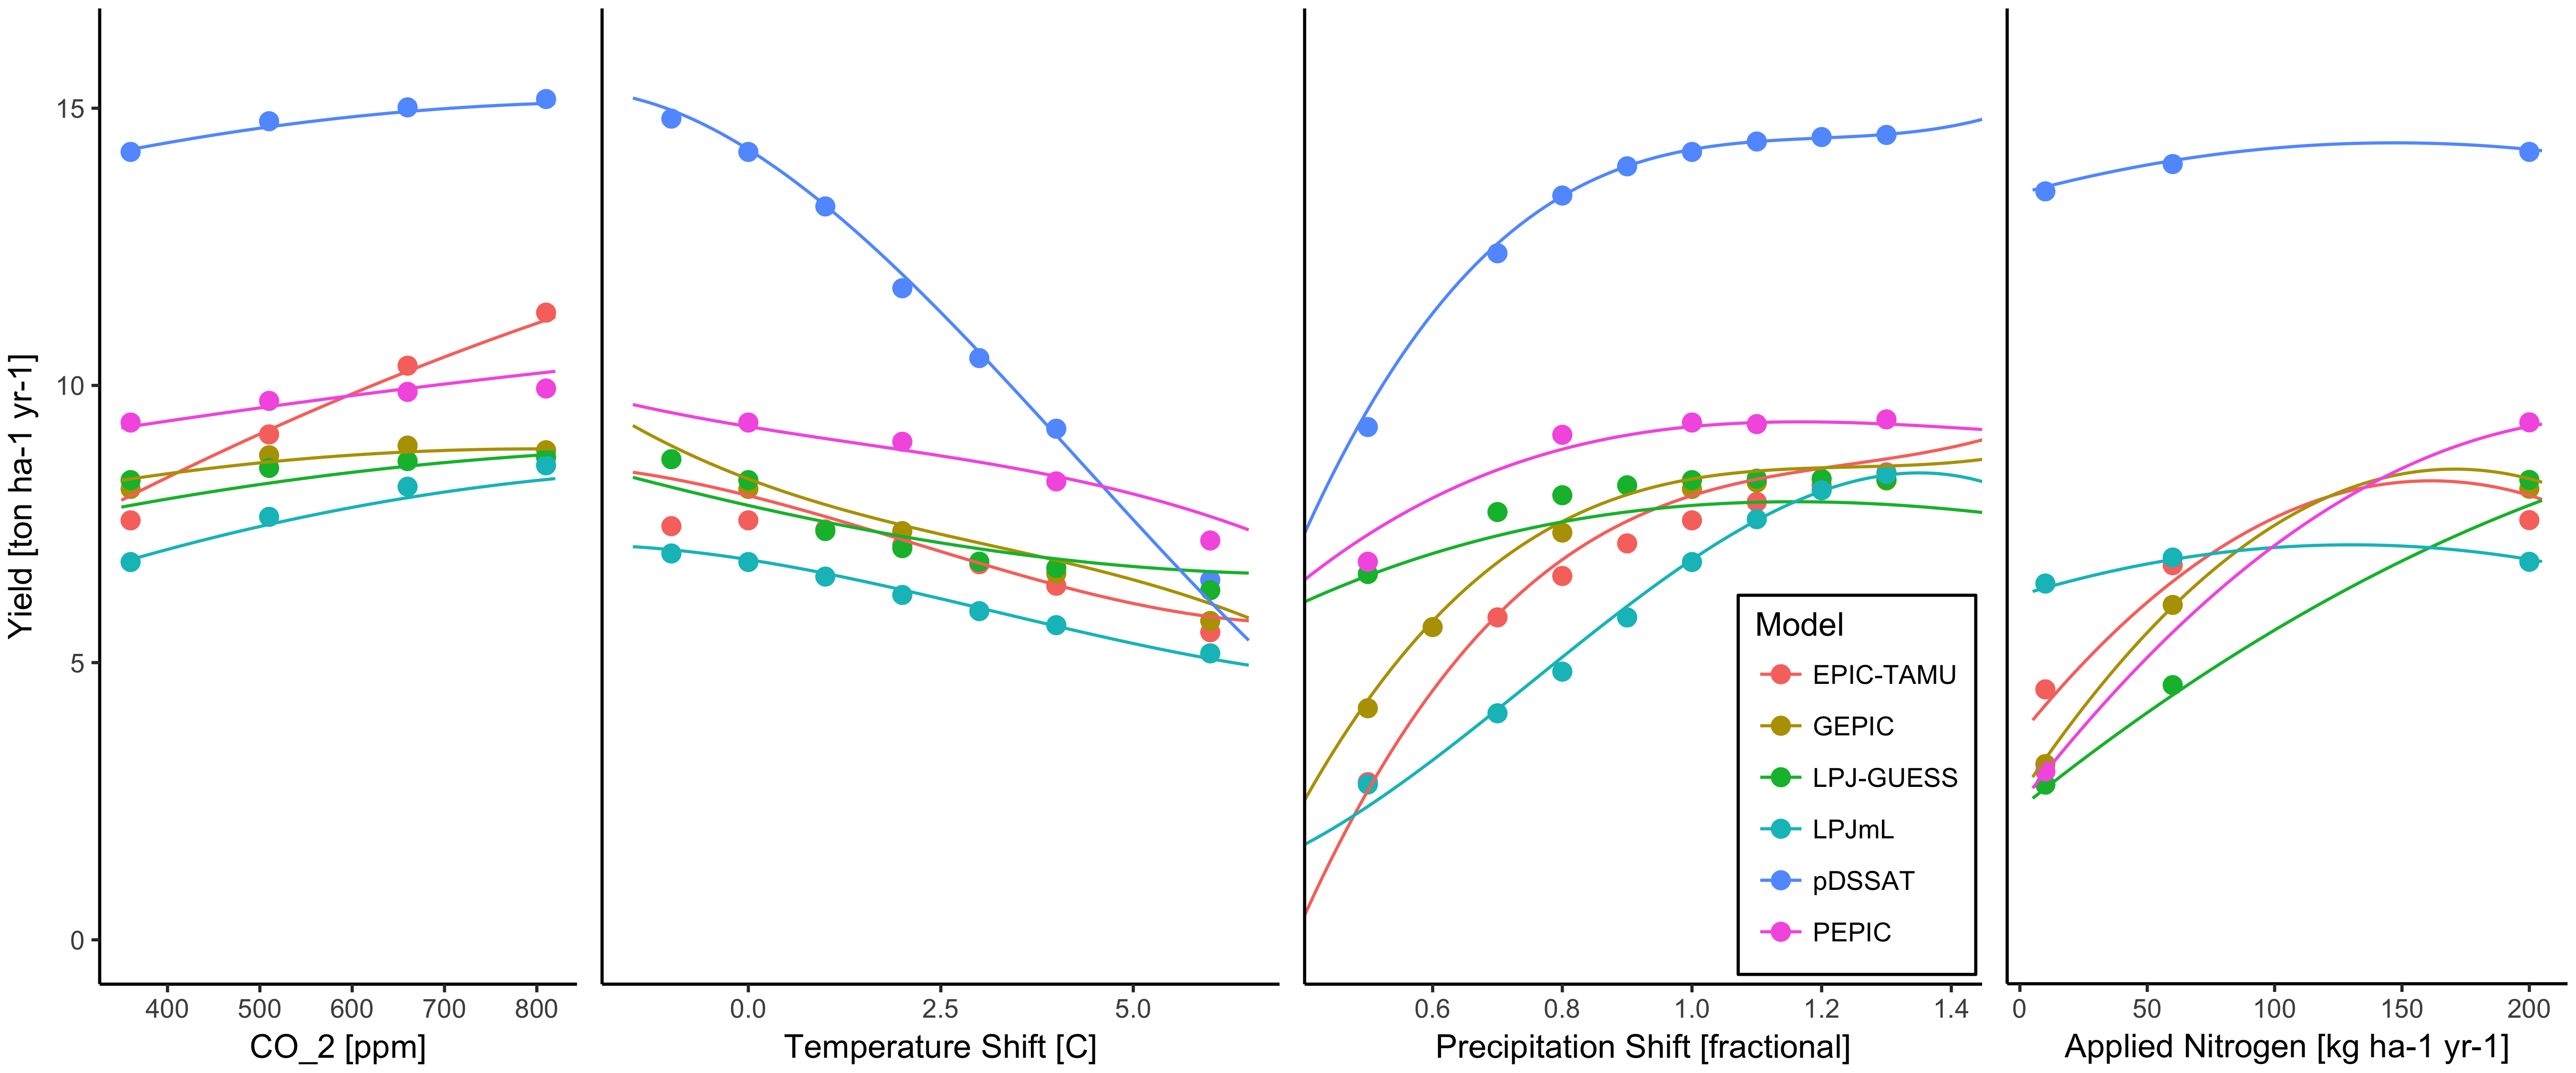
\includegraphics[width=0.95\linewidth]{figures/regression_model.png}
    \caption{Example illustrating across-model variations in yield response. We show simulations and emulations from six models for rain-fed maize in the same Iowa location shown in Figure \ref{fig:regression}, with the same plot conventions. Models that did not simulate the nitrogen dimension are omitted for clarity. The inter-model standard deviation is larger for the perturbations in CO$_2$ and nitrogen than for those in temperature or precipitation illustrating that the sensitivity to weather is better constrained than to management at elevated CO$_2$. While most model responses can readily emulated with a simple polynomial, some response surfaces are more complicated and lead to emulation error.}
   \label{fig:regression_iowa}
\end{figure*}

\subsection{Emulator performance}
Emulation provides not only a computational tool but a means of understanding and interpreting crop yield response across the parameter space. Emulation is only possible, however, when crop yield responses are sufficiently smooth and continuous to allow fitting with a relatively simple functional form. In the GGCMI simulations, this condition largely but not always holds. 
Responses are quite diverse across locations, crops, and models, but in most cases local responses are regular enough to permit emulation. Figure \ref{fig:regression} illustrates the geographic diversity of responses even in high-yield areas for a single crop and model (rain-fed maize in pDSSAT for various high-cultivation areas).  This heterogeneity validates the choice of emulating at the grid cell level. 

Each panel in Figure \ref{fig:regression} shows model yield output from scenarios varying only along a single dimension (CO$_2$, temperature, precipitation, or nitrogen addition), with other inputs held fixed at baseline levels; in all cases yields evolve smoothly across the space sampled. For reference we show the results of the full emulation fitted across the parameter space. The polynomial fit readily captures the climatological response to perturbations.

Crop yield responses generally follow similar functional forms across models, though with a spread in magnitude. Figure \ref{fig:regression_iowa} illustrates the inter-model diversity of yield responses to the same perturbations, even for a single crop and location (rain-fed maize in northern Iowa, the same location shown in the Figure \ref{fig:regression}). The differences make it important to construct emulators separately for each individual model, and the fidelity of emulation can also differ across models. This figure illustrates a common phenomenon, that models differ more in response to perturbations in CO$_2$ and nitrogen perturbations than to those in temperature or precipitation. (Compare also Figures \ref{fig:globesim} and \ref{fig:carbon}.) For this location and crop, CO$_2$ fertilization effects can range from $\sim$5--50\%, and nitrogen responses from nearly flat to a 60\% drop in the lowest-application simulation. 

While the nitrogen dimension is important and uncertain, it is also the most problematic to emulate in this work because of its limited sampling. The GGCMI protocol specified only three nitrogen levels (10, 60 and 200 kg~N y$^{-1}$ ha$^{-1}$), so a third-order fit would be over-determined but a second-order fit can result in potentially unphysical results. Steep and nonlinear declines in yield with lower nitrogen levels means that some regressions imply a peak in yield between the 100 and 200 kg~N y$^{-1}$ ha$^{-1}$ levels. While there may be some reason to believe over-application of nitrogen at the wrong time in the growing season could lead to reduced yields, these features are almost certainly an artifact of under sampling.In addition, the polynomial fit cannot capture the well-documented saturation effect of nitrogen application \citep[e.g.][]{Torsten77} as accurately as would be possible with a non-parametric model. 

\begin{figure}[!p]
\centering
    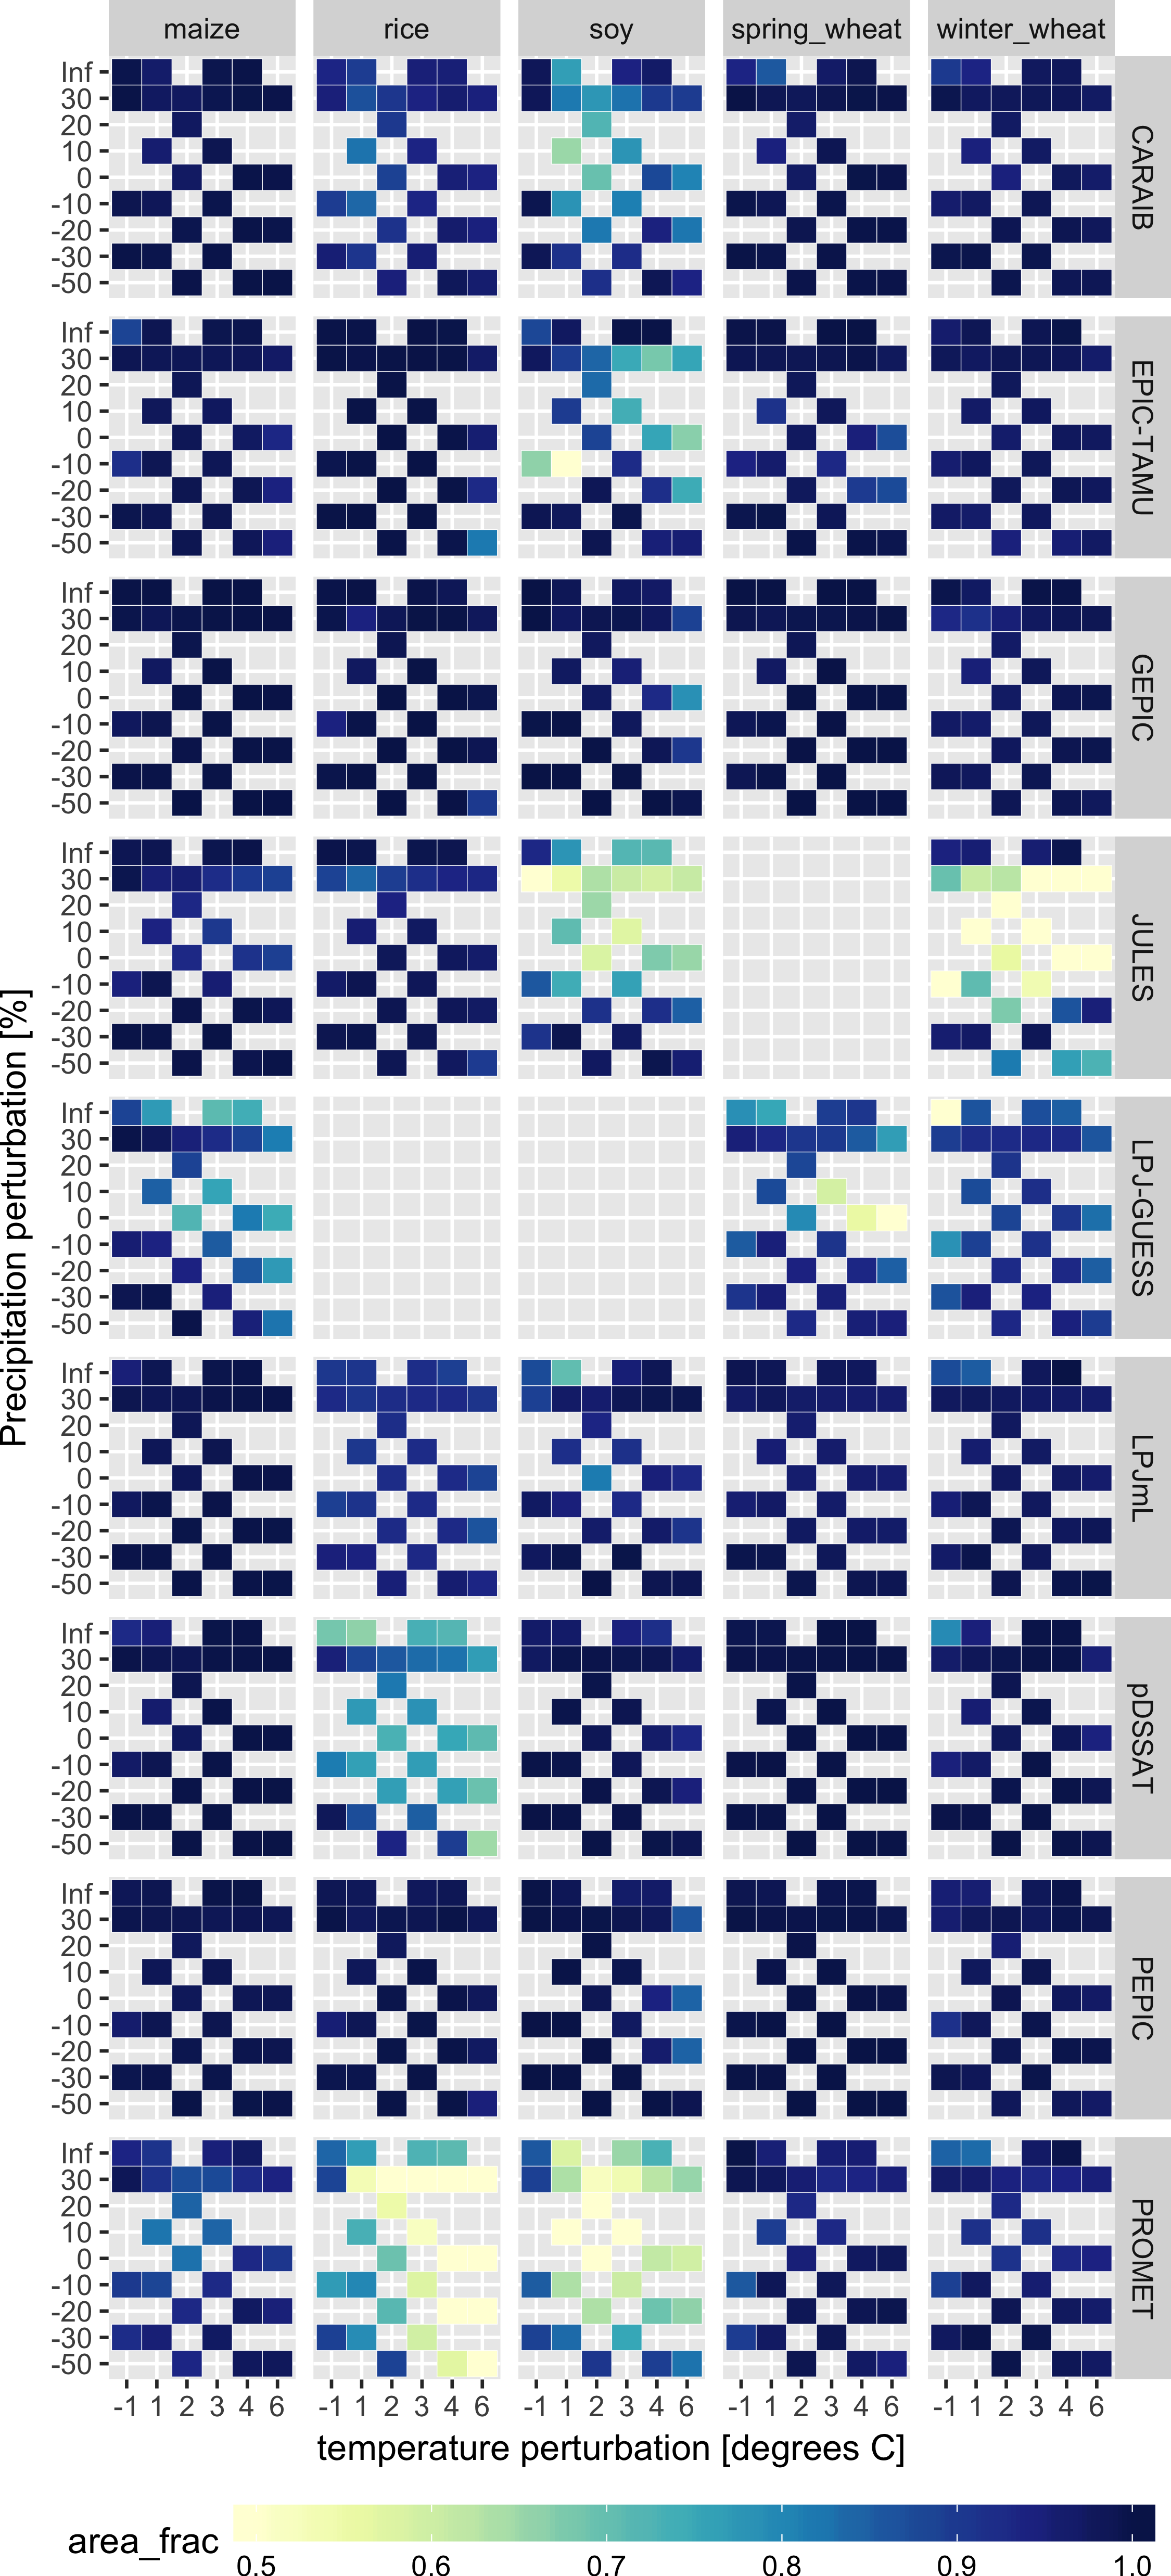
\includegraphics[width=1\linewidth]{figures/error_360.png}
    \caption{Assessment of emulator performance over currently cultivated areas based on normalized error (Equations \ref{eqn:error}, \ref{eqn:per_yield}). We show performance of all 9 models emulated, over all crops and all sampled T and P inputs, but with CO$_2$ and nitrogen held fixed at baseline values. Large columns are crops and large rows models; squares within are T,P scenario pairs. Colors denote the fraction of currently cultivated hectares with $ e < 1$.  Of the 756 scenarios with these CO$_2$ and N values, we consider only those for which all 9 models submitted data. JULES did not simulate spring wheat and LPJ-GUESS did not simulate rice and soy. Emulator performance is generally satisfactory, with some exceptions. Emulator failures (significant areas of poor performance) occur for individual crop-model combinations, with performance generally degrading for hotter and wetter scenarios.}
   \label{fig:error_360}
\end{figure}

\begin{figure}[!p]
\centering
    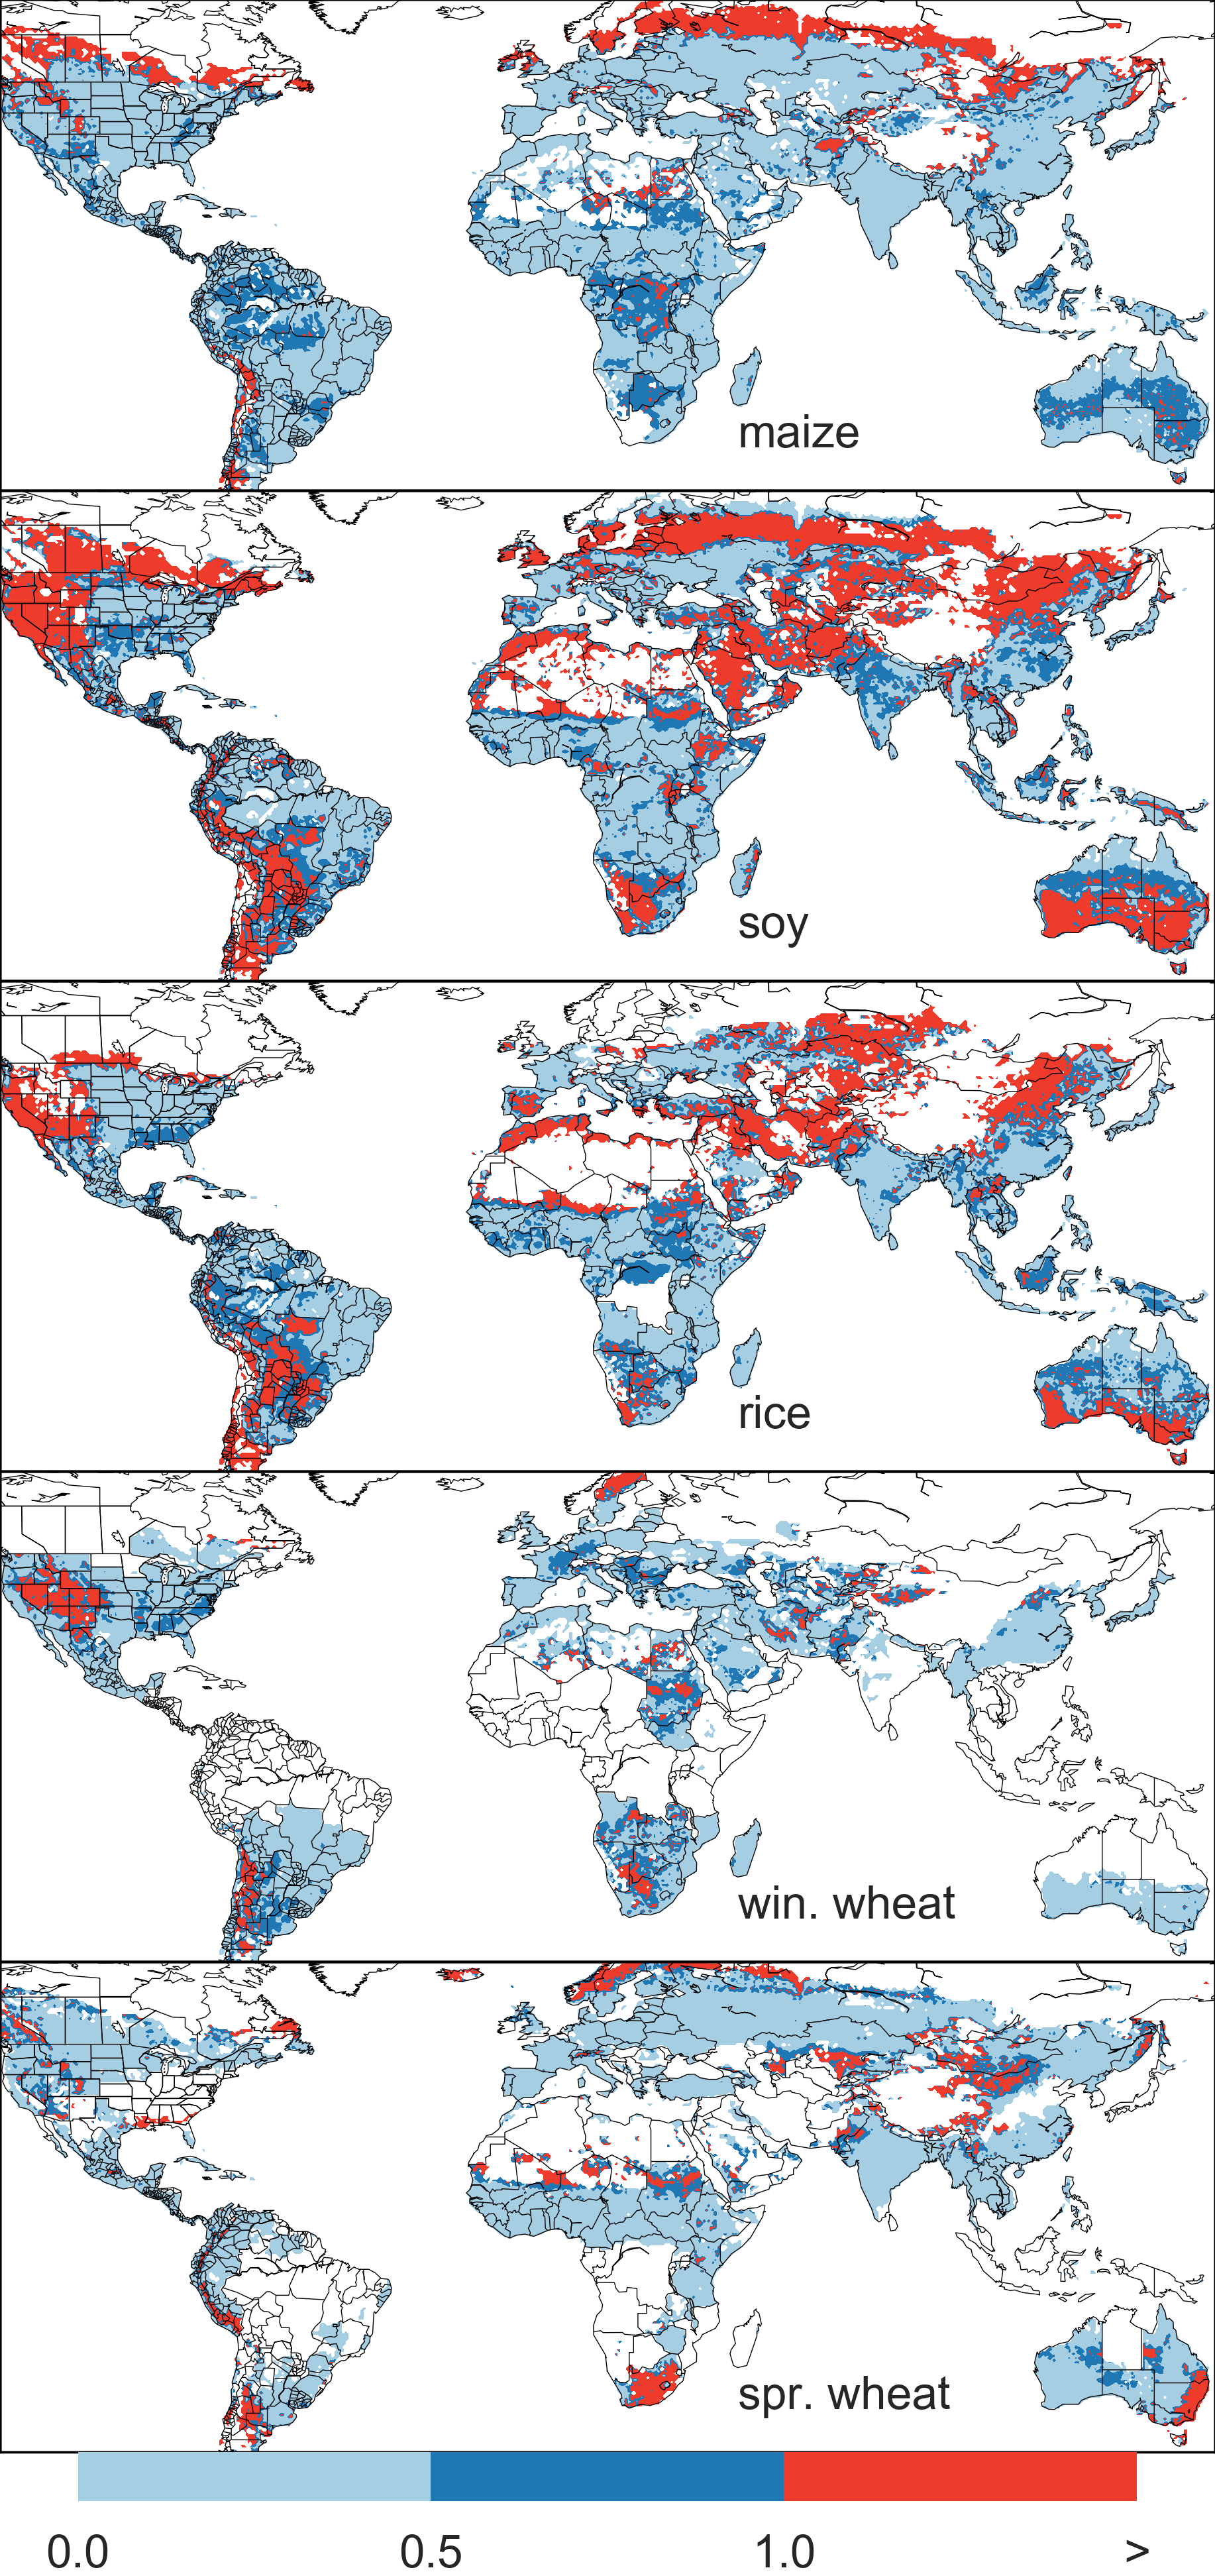
\includegraphics[width=0.95\linewidth]{figures/em_err.png}
    \caption{Illustration of our test of emulator performance, applied to the CARAIB model for the T+4 scenario for rain-fed crops. Contour colors indicate the normalized emulator error $e$, where $e > 1$ means that emulator error exceeds the multi-model standard deviation. White areas are those where crops are not simulated by this model. Models differ in their areas omitted, meaning the number of samples used to calculate the multi-model standard deviation is not spatially consistent in all locations. Emulator performance is generally good relative to model spread in areas where crops are currently cultivated (compare to Figure 1) and in temperate zones in general; emulation issues occur primarily in marginal areas with low yield potentials. For CARAIB, emulation of soy is more problematic, as was also shown in Figure \ref{fig:error_360}.}
   \label{fig:error}
\end{figure}

To assess the ability of the polynomial emulation to capture the behavior of complex process-based models, we evaluate the normalized emulator error. That is, for each grid cell, model, and scenario we evaluate the difference between the model yield and its emulation, normalized by the inter-model standard deviation in yield projections. This metric implies that emulation is generally satisfactory, with several distinct exceptions. Almost all model-crop combination emulators have normalized errors less than one over nearly all currently cultivated hectares (Figure \ref{fig:error_360}), but some individual model-crop combinations are problematic (e.g.\ PROMET for rice and soy, JULES for soy and winter wheat, Figures \ref{fig:errorjules}--\ref{fig:errorpromet}). Normalized errors for soy are somewhat higher across all models not because emulator fidelity is worse but because models agree more closely on yield changes for soy than for other crops (see Figure \ref{fig:temperature}, lowering the denominator. Emulator performance often degrades in geographic locations where crops are not currently cultivated. Figure \ref{fig:error} shows a CARAIB case as an example, where emulator performance is satisfactory over cultivated areas for all crops other than soy, but uncultivated regions show some problematic areas. 

It should be noted that this assessment metric is relatively forgiving. First, each emulation is evaluated against the simulation actually used to train the emulator. Had we used a spline interpolation the error would necessarily be zero. Second, the performance metric scales emulator fidelity not by the magnitude of yield changes but by the inter-model spread in those changes. Where models differ more widely, the standard for emulators becomes less stringent. Because models disagree on the magnitude of CO$_2$ fertilization, this effect is readily seen when comparing assessments of emulator performance in simulations at  baseline CO$_2$ (Figure \ref{fig:error_360}) with those at higher CO$_2$ levels (Figure \ref{fig:error810}). Widening the inter-model spread leads to an apparent increase in emulator skill.

\subsection{Emulator applications}
Because the emulator or ``surrogate model'' transforms the discrete simulation sample space into a continuous response surface at any geographic scale, it can be used for a variety of applications. Emulators provide a easy way to compare a ensembles of climate or impacts projections. They also provide a means for generating continuous damage functions. As an example, we show a damage function constructed from 4D emulations for aggregated yield at the global scale, for maize on currently cultivated land, with simulated values shown for comparison. (Figure \ref{fig:globe_em};  see Figures \ref{fig:temperature}- \ref{fig:nitrogen} in the supplemental material for other crops and dimensions.) The emulated values closely match simulations even at this aggregation level. Note that these functions are presented only as examples and do not represent true global projections, because they are developed from simulation data with a uniform temperature shift while increases in global mean temperature should manifest non-uniformly. The global coverage of the GGCMI simulations allows impacts modelers to apply arbitrary geographically-varying climate projections, as well as arbitrary aggregation mask, to develop damage functions for any climate scenario and any geopolitical or geographic level.

\begin{figure}[!htb]
    \centering
    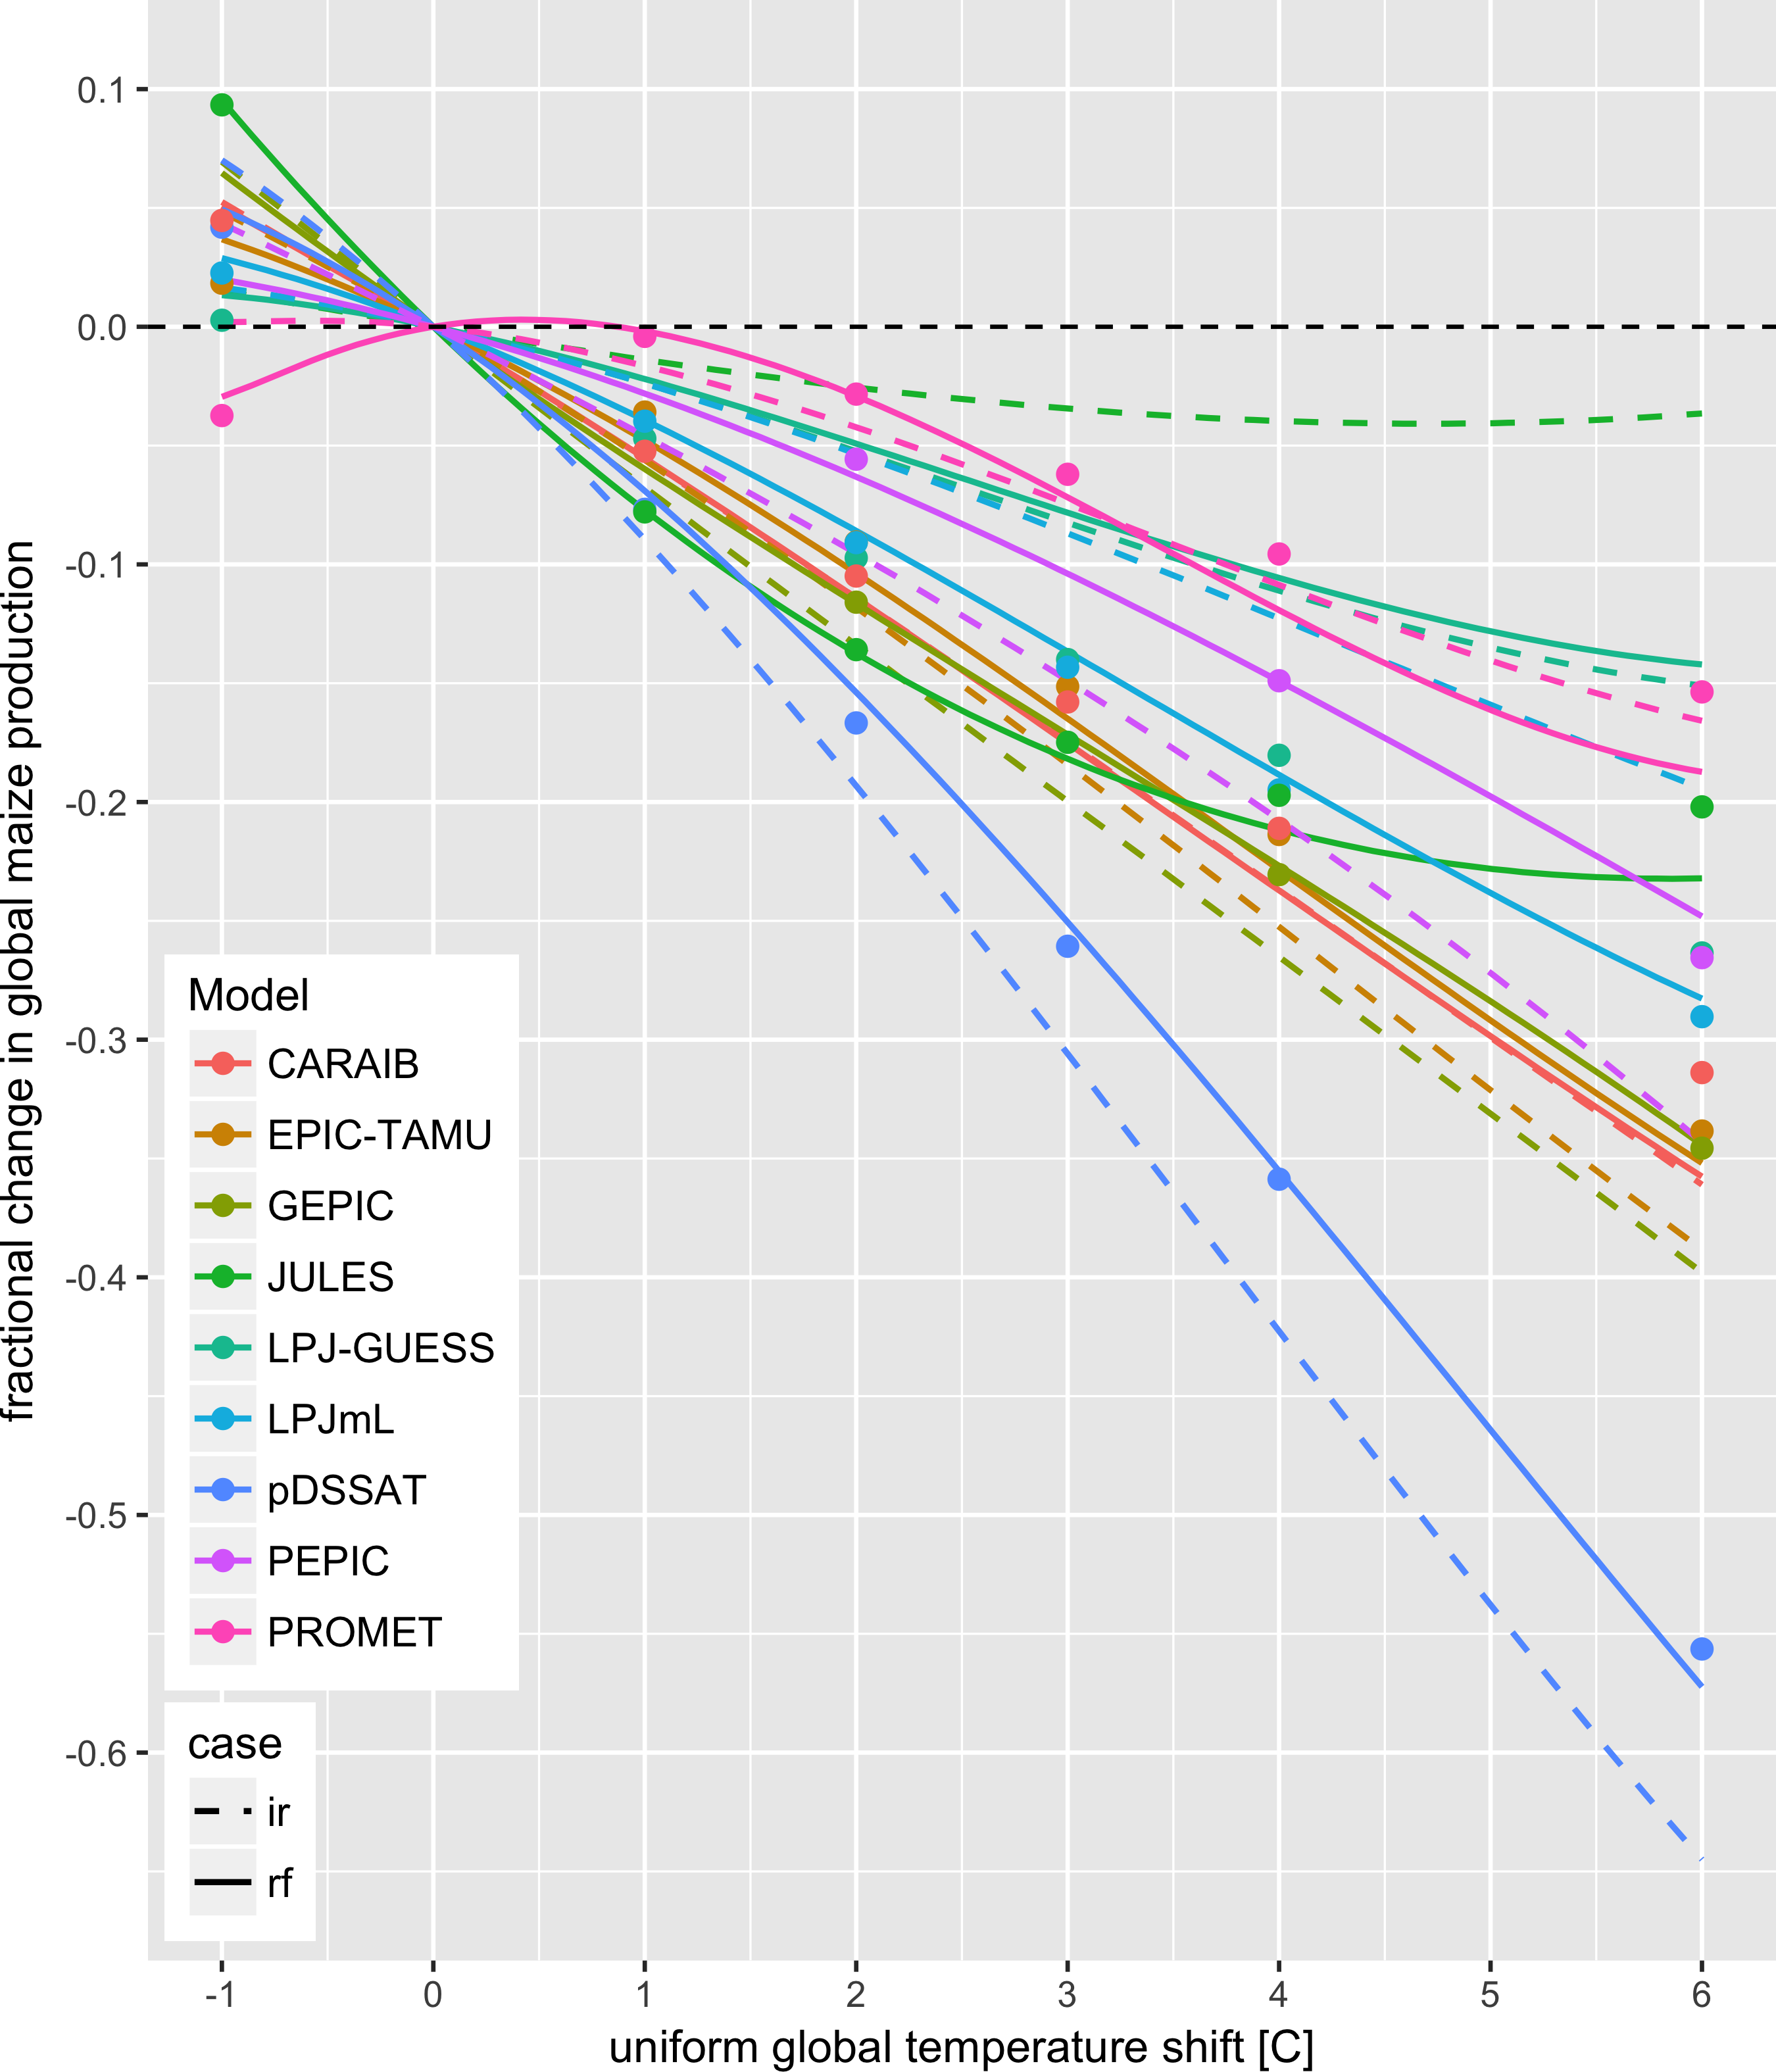
\includegraphics[width=0.95\linewidth]{figures/global_em_maize.png}
    \caption{Global emulated damages for maize on currently cultivated lands for the GGCMI models emulated, for uniform temperature shifts with other inputs held at baseline. (The damage function is created from aggregating up emulated values at the grid cell level, not from a regression of global mean yields.) Lines are emulations for rain-fed (solid) and irrigated (dashed) crops; for comparison, dots are the simulated values for the rain-fed case.  For most models, irrigated crops show a sharper reduction than do rain-fed because of the locations of cultivated areas: irrigated crops tend to be grown in warmer areas where impacts are more severe for a given temperature shift. (The exceptions are PROMET, JULES, and LPJmL.) For other crops and scenarios see Figures ~\ref{fig:temperature}- \ref{fig:nitrogen} in the supplemental material.}
    \label{fig:globe_em}
\end{figure}

\section{Conclusions and discussion} 
\label{S:4}
% -- summary of what was done
The GGCMI Phase II experiment assess sensitivities of process-based crop yield models to changing climate and management inputs, and was designed to allow not only comparison across models but evaluation of complex interactions between driving factors (CO$_2$, temperature, precipitation, and applied nitrogen) and identification of geographic shifts in high yield potential locations. While the richness of the dataset invites further analysis, we show only a selection of insights derived from the simulations. Across the major crops, inter-model uncertainty is greatest for wheat and least for soy. Across factors impacting yields, inter-model-uncertainty is largest for CO$_2$ fertilization and nitrogen response effects. Across geographic regions, inter-model uncertainty is largest in the high latitudes where yields may increase, and model projections are most robust in low latitudes where yield impacts are largest.  

Model performance when compared to historical data is mixed, with models performing better for maize and soy than for rice and wheat. The value of utilizing multiple models is illustrated by the distribution in performance skill across different countries and crops. An end-user of the simulation outputs or emulator tool may pick and choose models based on historical skill to provide the most faithful temperature and precipitation response depending on their application. The nitrogen and CO$_2$ responses were not validated in this work.

One counterintuitive result is that irrigated maize shows steeper yield reductions under warming than does rain-fed maize when considered only over currently cultivated land. The effect is the result of geographic differences in cultivated area. In any given location, irrigation increases crop resiliency to temperature increase, but irrigated maize is grown in warmer locations where the impacts of warming are more severe (Figures \ref{fig:KGirr_all}--\ref{fig:KGirr_currentcult}). The same behavior holds for rice and winter wheat, but not for soy or spring wheat (Figures \ref{fig:rice_currentcult}-\ref{fig:winter_wheat_currentcult}). Irrigated wheat and maize are also more sensitive to nitrogen fertilization levels, presumably because growth in rain-fed crops is also water-limited (Figure \ref{fig:nitrogen}). (Soy as a nitrogen-fixer is relatively insensitive to nitrogen, and rice is not generally grown in water-limited conditions.)

We show that emulation of the output of these complex responses is possible even with a relatively simple reduced-form statistical model and a limited library of simulations. Emulation therefore offers the opportunity of producing rapid assessments of agricultural impacts for arbitrary climate scenarios in a computationally non-intensive way. The resulting tool should aid in impacts assessment, economic studies, and uncertainty analyses. Emulator parameter values also provide a useful way to compare sensitivities across models to different climate and management inputs, and the terms in the polynomial fits offer the possibility of physical interpretation of these dependencies to some degree.

% -- caveats, future work --
%%%%%%%%%%%%%%
%%Needs Work%%
%%%%%%%%%%%%%%
We provide this simulation output dataset for further analysis by the community as we have only scratched the surface with this work. Each simulation run includes year to year variability in yields under different climate and management regimes. Some of the precipitation and temperature space has been lost due to the aggregation in the time dimension for the emulator presented here (i.e.\ the + 6 C simulation in the hottest year of the historical period compared to the coldest historical year, or precipitation perturbations in the driest historical year etc). Development of a year-to-year emulator or an emulator at different spatial scales may provide useful for some IAM applications. More exhaustive analysis of different statistical model specification for emulation will likely provide additional predictive skill over the specification provided here. The potentially richest area for further analysis is the interactions between input variable especially the Nitrogen and CO2 interactions with weather and with each other. More robust quantification of the sensitivity to the input drivers (and there differences across models), as well as quantification in differences in uncertainty across input drivers. Adaptation via growing season changes were also simulated and are available in the database, though this dimension was not presented or analyzed here.

The emulation approach presented here has some limitations. Because the GGCMI simulations apply uniform perturbations to historical climate inputs, they do not sample changes in higher order moments. The emulation therefore does not address the crop yield impacts of potential changes in climate variability. While some information could be extracted from consideration of year-over-year variability, more detailed simulations and analysis are likely necessary to diagnose the impact of changes in variance and sub-growing-season temporal effects. Additionally, the emulator is intended to provide the change in yield from a historical mean baseline value and should be used in conjunction with historical data (or data products) or a historical mean emulator (not presented here).

% -- summing up paragrah --
The future of food security is one of the larger challenges facing humanity at present. The development (and emulation) of multi-model ensembles such as GGCMI Phase II provides a way to begin to quantify uncertainties in crop responses to a range of potential climate inputs and explore the potential benefits of adaptive responses. Emulation also allow making state-of-the-art simulation results available to a wide research community as simple, computationally tractable tools that can be used by downstream modelers to understand the socioeconomic impacts of crop response to climate change. 

% Evidence for sharper fractional reduction in irrigated yields under increased temp when compared to rain-fed, 6 of the 9 models show this effect for maize, 4 of the 5 crops show this effect in the ensemble mean. See it in supp docs figure too for all regions, but clearly isn't the case when look at only currently cultivated land.
%Irrigated maize  For clarity, the irrigated simulations are not shown, but they follow the emulated paths closely with the JULES irrigated as the upper outlier. The sharper reduction in irrigated production is a consequence of the difference in cultivated area in the MIRCA2000 data set and generally higher baseline yields in the irrigated case.  As previously mentioned, irrigated crops are more resilient to temperature increase when analyzed on the global potential level.

%\item CO2 response - as expected is lower for maize (C4 vs C3) high CO$_2$ fixing efficiency for maize when compared to other crops \citep{Deryng2016}. large spread among models - each model represents the nutrient uptake and interaction process differently. response is greater for unirrigated because CO2 helps with water stress. % The responses to CO$_2$ when compared to the other drivers in these locations in the pDSSAT model is relatively flat. The pDSSAT response may be closer to reality than models than the models that show a strong CO$_2$ response for maize due to the ). The differences in CO$_2$ and nitrogen respose across models is a direct result of the fact that 

%can be compared locally or aggregated up to any level for comparison purposes that go beyond just comparison of specific scenario yields. 
%The interaction term coefficients are of special interest, and the emulations presented here allow exploration of questions such as CO$_2$ response under nitrogen stress, and potential changing efficacy of nitrogen fertilization under conditions of severe climate change.
% because they distill the relative importance that applied fertilizers have under a changing climate. The research team has more investigation planned in this domain.

% --- tools actually available ----
%All results and outputs from the GGCMI Phase II exercise are available to the public. Parameter values for a single case are available in 3D arrays ranging in size from 12MB (no nitrogen irrigated case) to 49MB (nitrogen included rain-fed case). Calculating yields involves passing 0.5 degree resolution arrays of temperature and precipitation deviations from historical climatology (in $^{\circ}$C and percent difference respectively), as well as an applied nitrogen array and a global CO$_2$ scalar into Equation \ref{eqn:features_final}. Any post processing area aggregation and cultivation weights desired can then be applied. Impact modelers can use the emulator to develop a damage function (or benefit function) at any spatial scale larger than 0.5 degree Latitude and Longitude. or integrate the polynomial directly into an existing framework. Caution that the emulator is intended be be used with actual climate changes, not uniform offsets 

%Comparing a non-physical linear daily temperature and precipitation perturbations to mean climatological yields is likely m More work is required to better understand these relationships.
% The nitrogen dimension proves to be especially difficult to represent with the polynomial model. Additional applied nitrogen simulation levels would be beneficial for future improvements to the emulator.


\section{Acknowledgments}
\label{S:5}
We thank Michael Stein and Kevin Schwarzwald, who provided helpful suggestions that contributed to this work. This research was performed as part of the Center for Robust Decision-Making on Climate and Energy Policy (RDCEP) at the University of Chicago, and was supported through a variety of sources. RDCEP is funded by NSF grant \#SES-1463644 through the Decision Making Under Uncertainty program. J.F.\ was supported by the NSF NRT program, grant \#DGE-1735359. C.M.\ was supported by the MACMIT project (01LN1317A) funded through the German Federal Ministry of Education and Research (BMBF).  C.F.\ was supported by the European Research Council Synergy grant \#ERC-2013-SynG-610028 Imbalance-P. P.F. and K.W. were supported  by the Newton Fund through the Met Office Climate Science for Service Partnership Brazil (CSSP Brazil). A.S.\ was supported by the Office of Science of the U.S. Department of Energy as part of the Multi-sector Dynamics Research Program Area. Computing resources were provided by the University of Chicago Research Computing Center (RCC). S.O.\ acknowledges support from the Swedish strong research areas BECC and MERGE together with support from LUCCI (Lund University Centre for studies of Carbon Cycle and Climate Interactions).
\section{References}
\label{S:6}

%% \appendix
%% \section{}
%% \label{}

%% References
%% Following citation commands can be used in the body text:
%% Usage of \cite is as follows:
%%   \cite{key}          ==>>  [#]
%%   \cite[chap. 2]{key} ==>>  [#, chap. 2]
%%   \citet{key}         ==>>  Author [#]
\bibliography{bib.bib}

%\printbibliography
%% References with bibTeX database:
%% Authors are advised to submit their bibtex database files. They are requested to list a bibtex style file in the manuscript if they do not want to use model1-num-names.bst.

\end{document}
%% End of file `elsarticle-template-1-num.tex'.

%%%%%%%%%%%%%%%%%%%%%%%%%%%%%%%%%%%%%%%%%%%%%%%%%%%%%%%%%%%%%%%%
%%%%%%%%%%%%%%%%%%%%%%%%%%%%%%%%%%%%%%%%%%%%%%%%%%%%%%%%%%%%%%%%
%%%%%%%%%%%%%%%%%%%%%%%%%%%%%%%%%%%%%%%%%%%%%%%%%%%%%%%%%%%%%%%%
%%%%%%%%%%%%%%%%%%%%%%%%%%%%%%%%%%%%%%%%%%%%%%%%%%%%%%%%%%%%%%%%
% notes from Liz

%there are a lot of results in Conclusions/Discussion, some of which are only thinly discussed - might get asked to move them or justify more. (Unless you moved these already)

%- why not compare your emulator to statistical models from others?  You might say because models weren't calibrated, but it's a reasonable and may have to be addressed.

%- if we didn't state the irrigated/unirrigated conclusion in the abstract, we should do that

%- on irrigated/unirrigated figures in supp docs - for the currently cultivated land, put the mean temp for the relevant area for irrigated and unirrigated, to back up assertion in paper that there is a temperature difference.

%- We claimed that irrigated damages were higher because damages for a given T change are larger for a given baseline temperature. Is that backed up in the paper? Only indirectly by the maps that show stronger damages in the T+4 case for low latitudes than high latitudes. It could be interesting to do scatterplot of yield changes for a given scenario where the x axis is baseline climate. (Or include two scenarios colored differently...)

%- probably good to explain in more detail that simpler fitting methods can cause problems. Even just a sentence or two in the main manuscript to explain that your choice is better. If you wanted to put in the results of more methodological work, that could work too, either in the main paper or the supp docs. Part of the paper's message is that emulation is possible; it would make sense to explain that it is NOT possible to emulate well if you don't use the right approach.

%%%%%%%%%%%%%%%%%%%%%%%%%%%%%%%%%%%%%%%%%%%%%%%%%%%%%%%%%%%%%%%%
%%%%%%%%%%%%%%%%%%%%%%%%%%%%%%%%%%%%%%%%%%%%%%%%%%%%%%%%%%%%%%%%
%%%%%%%%%%%%%%%%%%%%%%%%%%%%%%%%%%%%%%%%%%%%%%%%%%%%%%%%%%%%%%%%
%%%%%%%%%%%%%%%%%%%%%%%%%%%%%%%%%%%%%%%%%%%%%%%%%%%%%%%%%%%%%%%%
